%%%%%%%%%%%%%%%%%%%%%%%%%%%%%%%%%%%%%%%%%%%%%%%%%%%%%%%%%%%%%%%%%%%%%%
% LaTeX Template: Project Titlepage
%
% Source: http://www.howtotex.com
% Date: April 2011
% 
% This is a title page template which be used for articles & reports.
% 
% Feel free to distribute this example, but please keep the referral
% to howtotex.com
% --------------------------------------------------------------------
% Preamble
% --------------------------------------------------------------------
\documentclass[paper=a4, fontsize=11pt,twoside]{scrartcl}	% KOMA

\usepackage[a4paper,pdftex]{geometry}	% A4paper margins
\setlength{\oddsidemargin}{5mm}			% Remove 'twosided' indentation
\setlength{\evensidemargin}{5mm}
\setlength{\parindent}{0pt}
\usepackage{pdfpages}
\usepackage[english]{babel}
\usepackage{listing}
\usepackage[protrusion=true,expansion=true]{microtype}	
\usepackage{amsmath,amsfonts,amsthm,amssymb}
\usepackage{graphicx}
\usepackage{float}
\usepackage{fancyvrb}
\usepackage{blindtext}
\usepackage{listings}
\usepackage{enumitem}
\usepackage{longtable}
\usepackage{titling}\graphicspath{{img/}}
\usepackage{xpatch}

%Define the listing package
\usepackage{listings} %code highlighter
\usepackage{color} %use color
\definecolor{mygreen}{rgb}{0,0.6,0}
\definecolor{mygray}{rgb}{0.5,0.5,0.5}
\definecolor{mymauve}{rgb}{0.58,0,0.82}
 
%Customize a bit the look
\lstset{ %
backgroundcolor=\color{white}, % choose the background color; you must add \usepackage{color} or \usepackage{xcolor}
basicstyle=\footnotesize, % the size of the fonts that are used for the code
breakatwhitespace=false, % sets if automatic breaks should only happen at whitespace
breaklines=true, % sets automatic line breaking
captionpos=b, % sets the caption-position to bottom
commentstyle=\color{mygreen}, % comment style
deletekeywords={...}, % if you want to delete keywords from the given language
escapeinside={\%*}{*)}, % if you want to add LaTeX within your code
extendedchars=true, % lets you use non-ASCII characters; for 8-bits encodings only, does not work with UTF-8
frame=single, % adds a frame around the code
keepspaces=true, % keeps spaces in text, useful for keeping indentation of code (possibly needs columns=flexible)
keywordstyle=\color{blue}, % keyword style
% language=Octave, % the language of the code
morekeywords={*,...}, % if you want to add more keywords to the set
numbers=left, % where to put the line-numbers; possible values are (none, left, right)
numbersep=5pt, % how far the line-numbers are from the code
numberstyle=\tiny\color{mygray}, % the style that is used for the line-numbers
rulecolor=\color{black}, % if not set, the frame-color may be changed on line-breaks within not-black text (e.g. comments (green here))
showspaces=false, % show spaces everywhere adding particular underscores; it overrides 'showstringspaces'
showstringspaces=false, % underline spaces within strings only
showtabs=false, % show tabs within strings adding particular underscores
stepnumber=1, % the step between two line-numbers. If it's 1, each line will be numbered
stringstyle=\color{mymauve}, % string literal style
tabsize=2, % sets default tabsize to 2 spaces
title=\lstname % show the filename of files included with \lstinputlisting; also try caption instead of title
}
%END of listing package%
 
\definecolor{darkgray}{rgb}{.4,.4,.4}
\definecolor{purple}{rgb}{0.65, 0.12, 0.82}
 
%define Javascript language
\lstdefinelanguage{JavaScript}{
keywords={typeof, new, true, false, catch, function, return, null, catch, switch, var, if, in, while, do, else, case, break},
keywordstyle=\color{blue}\bfseries,
ndkeywords={class, export, boolean, throw, implements, import, this},
ndkeywordstyle=\color{darkgray}\bfseries,
identifierstyle=\color{black},
sensitive=false,
comment=[l]{//},
morecomment=[s]{/*}{*/},
commentstyle=\color{purple}\ttfamily,
stringstyle=\color{red}\ttfamily,
morestring=[b]',
morestring=[b]"
}
 
\lstset{
language=JavaScript,
extendedchars=true,
basicstyle=\footnotesize\ttfamily,
showstringspaces=false,
showspaces=false,
numbers=left,
numberstyle=\footnotesize,
numbersep=9pt,
tabsize=2,
breaklines=true,
showtabs=false,
captionpos=b
}
% --------------------------------------------------------------------
% Definitions (do not change this)
% --------------------------------------------------------------------
\newcommand{\HRule}[1]{\rule{\linewidth}{#1}} 	% Horizontal rule
\newcommand\tab[1][1.4cm]{\hspace*{#1}}
%\makeatletter							% Title
%\def\printtitle{%						
%    {\centering \@title\par}}
%\makeatother									
\makeatletter							% Author
\def\printauthor{%					
    { \large \@author}}				
\makeatother							
\usepackage{titling}

\setlength{\droptitle}{-10em}   % This is your set screw
\title{\huge Logbooking Software for Science}




\begin{document}
\lstset{language= Java}

% ------------------------------------------------------------------------------
% Maketitle
% ------------------------------------------------------------------------------
\thispagestyle{empty}		% Remove page numbering on this page
\maketitle
\vspace{2cm}
\begin{figure}[H]
\centering

\includegraphics[scale=0.5]{alice}
\end{figure}

\vspace{4cm}
\begin{longtable}{  p{4cm}  p{8cm} }
Author: & F.P. van der Meulen \\
Internship Supervisor: & C.J. Rijsenbrij
\end{longtable}
\thispagestyle{empty}

\newpage 
\begin{longtable}{  p{8cm}  p{8cm} }
Student: & F.P. van der Meulen \\
StudentNumber: & 500713781 \\
Phone Number: & +31 6 17506168 \\
\\
Place: & Amsterdam, the Netherlands \\
Date: & August 16th \\
\\
Institution: & Amsterdam University of Applied Sciences \\
Study course: & HBO-ICT (Game Development) \\
Internship Supervisor: & C.J. Rijsenbrij \\
\\
Organization: & Software for Science \\
Address: & Weesperplein 2-4 \\
 & 1091 GM Amsterdam \\
Company supervisor: & Dr. Marten Teitsma \\
Phone number: & +31 6 21156982\\
\\
Internship Period: & Semester 2, 2018 

\end{longtable}
\newpage



\newpage
\tableofcontents

\newpage
\section*{Preface}
I would like to thank the following persons:

Dr. Marten Teitsma for allowing me to work on this project. He has peaked my interest in programming for scientific projects, and I hope that I can continue this path of programming.\\
Heiko van der Heijden for his help with programming matters and on giving advise on how to improve my code. You have improved my knowledge about programming tremendously. \\
Kees Rijsenbrij for helping me with setting up my thesis. Your advise has helped me a lot on making this thesis as the way it is now. \\
Naomi Nazar for helping with deciding which requirements would be implemented into the prototype. \\
Pascal Boeschoten for clarifying the vague and unknown terms that were in the requirement document.


\newpage
\section*{Abstract}
This thesis internship took place at Software for Science. Software for Science works alongside scientific organizations to create load balancing software and monitoring system software for these scientific organizations. One of the scientific organizations, CERN, wanted a new bookkeeping system to replace the one that was in use. For this, a prototype was required, combining the predefined wishes from CERN with the learning possibilities for Software for Science in a limited amount of time. This thesis investigated which of CERN's requirements could be established into the prototype. \\ 
After reading CERN's requirement documents, it was discovered that there were some requirements that were unclear and vague. Also, it was found that some requirements were mentioned multiple times in the same document, which needed to be grouped together to prevent duplicity. The analysis method was used is the A.H.P. and the Hierachy A.H.P. method. This method gives a score to each requirement based upon pre-defined criteria. \\
Once the analysis was completed, the requirements with the lowest score were removed form the list. Choosing the eventual requirements was done with the help of front-end developer Naomi, Software for Science and CERN itself. \\ 
Before the prototype was being developed, frameworks, modules, design patterns and programming languages were chosen to realise the prototype of the bookkeeping system. In the end, the design patterns Singleton and the Model View Controller are chosen, the programming language will be JavaScript, the framework will be CERN's own ALICE-WebUI for creating the server and the modules would be chosen during development. \\
To prove that the prototype is working as intended, test cases were created to test the prototype. To verify that these test cases were executed, the test cases were converted into programmed tests. 
The vague and unclear requirements were made clear with the help of interviewing a former shifter, Pascal Boeschoten. The requirements were analysed and as a result lists of prioritized requirements were created, ordered by feature and the duplicate requirements were grouped together. \\
With the help of the list of prioritized requirements, the front-end, CERN and S.F.S, requirements could be chosen to be featured in the prototype with an extra requirement that depended on a piece of software from CERN. 
By combining the different frameworks, design patterns, modules and the list of chosen requirements, a prototype was made. Not all requirements and a planned design pattern could be implemented in the prototype. This had to do either with time constraints(the requirements were bigger than expected) or the use of special technology which would take too much time to complete(setting up an email server). \\
The test cases were created based upon a list of possible scenarios that were created. The test cases were then verified with creating the  programmed tests. As a result, the tests have verified that the prototype is working as intended. \\
The requirements that were implemented into the prototype were requirements about creating log entries, uploading files to log entries and about a user login. 
 



\newpage
\section{Introduction}
This is a student thesis from the Amsterdam University of Applied Sciences from the HBO-ICT Game Development study course. The thesis took place at Software for Science. \\
Software for Science is an organization, lead by Dr. Marten Teitsma, that is involved with scientific experiments. Software for Science creates software for multiple scientific experiments, such as software for load balancing and monitoring systems for scientific organizations. Software for Science is created as an organization from the Amsterdam University of Applied Sciences. Software for Science works together with scientific organizations such as Astron(the Netherlands Institute for Radio Astronomy), eScience center(the Dutch national center of excellence for the development and application of research software to advance academic research) and CERN(Conseil Européen pour la Recherche Nucléaire). \\
CERN is a scientific research center in Geneva, Switzerland, focused on researching nuclear energy and inventing new technologies, such as the predecessor of the internet. CERN works with particle colliders for their nuclear research, e.g., shooting particles against each other in order to find out what energy, atoms and other substances comes free from one of those runs. CERN works with multiple particle colliders to create new particles, or to research events that has happened in the past, such as the big bang. One of those particle colliders is ALICE. \\
ALICE, A Large Ion Collider Experiment, is a particle detector that detects particles of the other particle colliders. ALICE consists of many sub parts, called subsystems. Every time that the particle colliders are running and when ALICE detects something, it is being recorded as a run in ALICE's own bookkeeping system. This bookkeeping system makes sure that the runs ALICE detects are recorded into the bookkeeping system so that researchers, collaborators with CERN and external people can look back upon the runs. This also includes reports whenever a shifter, a scientist or student that analyses a run from ALICE, has completed their shift and need to write down what the shifter did during their shift. Other kind of reports are the reports about incidents with ALICE, reports about filling the gas and reports that ALICE itself makes, for example, when a run takes place, it automatically records all the details of the run. In December of 2018, ALICE is going under maintenance. CERN calls it a long shutdown. During the maintenance, subsystems and parts of ALICE are being renewed. Before the maintenance started, the request for a new bookkeeping system was made. \\

\newpage
\section{The assignment}
There are three reasons for a new bookkeeping system that CERN have been given. The first reason is that the new system must combine the bookkeeping system with AliMonitor, a existing monitoring system. The second reason is that there are multiple desired features that are not added to the current system. One of those features is creating log entries using a predefined template to have consistent log entries. The third reason is that most of the technologies and frameworks used to develop the system is outdated due to the fact that development started around 2009. From 2009 until now, new features were added to the system and new tables were created in the database. This made the code- and database structure difficult to maintain. \\ \\
Software for Science is planning to deliver the new bookkeeping system in January. Before the start of the development of the actual bookkeeping system, they plan to show a prototype of the bookkeeping system in June to CERN software developers and users that are involved with the current bookkeeping system. The reason why a prototype needs to be created is that Software for Science wants to learn more about creating a bookkeeping system. With the prototype, it will be easier to detect possible flaws when creating the actual bookkeeping system, since with the prototype, a similar bookkeeping system has been created and it is possible to experiment with new technologies that could be useful for the actual bookkeeping system. \\ \\
After the prototype is developed and demonstrated at CERN, Software for Science hosts a summer school, a special program for international students that are interested in developing software for scientific research. At the summer school, the students will work with the prototype to let them learn more about combining science with software. The students will experiment and work with the prototype of the bookkeeping system. Finally, at September of 2018, a semester at the University of Applied Sciences will be dedicated to create the actual bookkeeping system. \\ \\ 
Due to the size of the project, the time constraints that are involved, and the many requirements that CERN has given for the actual product, not every requirement and feature can be implemented into the prototype. Furthermore, it is important that possible flaws with the chosen requirements can be detected as early as possible. Based upon the current situation, the following research question can be formulated: \\ \\
\textit{Which requirements can be implemented into the logbook system for ALICE?}
\\ \\
In order to make a prototype for the new bookkeeping system, the back end and the front end are separated from each other. This was done due to the fact that the scope of the project would become too big and thus there would be less requirements implemented into the prototype. The second reason why the front end and the back end are separated is that the front end and the back end will run on different machines. While the back end will run on a server, the front end must run on every computer at CERN in June. This thesis will be about the back end of the new bookkeeping system. The front end will be developed by Naomi Nazar.
\\ 
This thesis is split into four parts. Every part consists a sub research question. An explanation why these sub research questions are important and how they could help solving the main research question can be found later in the thesis. The sub research questions are as followed: \\
\begin{enumerate}
\item \textit{Which requirements are important for the logbook system for ALICE?}
\item \textit{What are the consequences for the development process of the prototype based upon the important requirements and the database choices?}
\item \textit{How can the prototype be developed?}
\item \textit{Which test cases verify that the prototype works?}
\end{enumerate}
The second research question will be completed with the help of front end developer Naomi since the front end needs to design and create the look of the prototype. \\
Based upon the results from the research questions, a bookkeeping prototype can be created. The prototype will be demonstrated to the developers at CERN. The prototype will be delivered with the thesis as a code project. 

 

%\newpage
%\section{Techniques}
%This chapter will discuss the different techniques that were used to create the prototype and the thesis. 

%\subsection{ Node JavaScript}
%The main programming language for this research is Node JavaScript. Node JavaScript is a hard set requirement, e.g. the project must use JavaScript on the back and the front end. The version of Node that is used is version 9.4.0. At the start of the development, this was the most recent version of node JavaScript that was used.

%\subsection{Travis CI}
%Travis CI is a continues integrated testing tool [5]. It is used to test commits that a developer makes to the git repository. It will run all the tests that are available and sends an email whenever tests that were made earlier fails. This tool is used for maintaining the quality of the prototype.

%\subsection{Sublime text 3}
%The development environment for developing the prototype is Sublime Text 3 [6]. Sublime text is an simple Integrated Development Environment, and stills offers all the important tools and features that would be needed for developing the back end. This was the Environment that was used to create the prototype.

%\subsection{Lucichart}
%Lucichart[12]is used for the creation of the Entity Relation Diagram's and the Unified Modelling Language Diagrams. This tool is an online based diagram creator and offers templates for the type of diagram that the user needs.  

%\subsection{Scrum}
%Scrum[7] is the work management method that is used for the development of the prototype. Both the front end and the back end make use of this work management method. With scrum, sprints are created to develop features on the according time. The final four sprints of the prototype will be discussed later in the thesis.  

%\subsection{Git}
%Git has been used as the version control system for the prototype and for the thesis. With Git, it was possible to store the code online, making sure it was always available for use on any computer. This is the same case for the thesis.

\newpage


\section{Methods}
This chapter discusses the methods used to solve the research questions. The four research questions that were earlier created will be discussed, further explained and at the end of each section, a summary will be given on how to approach and resolve every research question. The order of solving the research questions are as written down earlier.\\
The first step is to analyse all the requirements from the requirements document involving the bookkeeping system. Once the analysation is completed,  a list of requirements that can be implemented into the prototype can be made. The prototype will be then developed with the help of predefined programming languages and possible design patterns, frameworks and modules.Finally, the prototype will be tested to verify that the prototype is working. \\
These summaries will be also given at the beginning of each results section, so that is explained how the research question will be answered.

\newpage
\subsection{Req analysis}
This section of the thesis will discuss the requirements analysis. There are over 120 requirements created by CERN and  Software for Science helped with formulating these requirements. These requirements were made before the start of the thesis. Due to the size of the requirements document, this will be a source rather than an attachment. It is impossible to use every requirement in the prototype, due to scale of the requirements and due to time constraints that are set. An analysis is needed in order to check which requirements are necessary to add to the prototype and which requirements can be left out.  \\
Inside the requirement document are some vague terms that aren't explained. The terms are follow-ups, on call intervention, announcements, and an EOS report. These vague terms will create confusion when prioritizing the requirements. And that will cause that important features could be left out of the prototype. \\ \\
Furthermore, there are requirements about placing comments under log entries. It is unclear however on how extended placing comments under log entries are. The best way to make it clear is to either receive this information from CERN or to conduct an interview with someone from CERN.  \\ 
Software for Science has also given criteria for the prototype. This criteria is that all the requirements related to the Subsystem Run Coordinator must be added to the prototype. This criteria will be crucial for the requirement analysis. \\ \\
The technique that will be used for the requirement analysis is the Analytic Hierarchy Process technique.[9] "In A.H.P., initially whole requirements are recognized and then criteria under which these requirements will be preferred. In A.H.P. we pair wise analysing  between  the  probable  pairs  of  the  hierarchy. 
Now users can recognize the possible relationship between 
the hierarchies. We then pair wise analyse them and users can select its preferences from the scale which ranges from 
one to nine."(Javed Ali Khan et all, 2015). The second software requirements analysis technique that will be used for the software is the Hierachy Analytic Hierachy Process technique[9]. H.A.H.P. is a technique that creates so called planes of requirements in order to simplify the requirement analysis process. A plane is a group of requirements that are grouped together if they share a similarity. These planes can, for example, align to a user of the system or a feature that will be implemented into the final product. For this requirement analysis, the planes will consist of features since this will be more important for the prototype than the users themself. \\ \\
The last criteria that will be used for the analysis is time. Time is an important factor for the requirement analysis, due to the limited time available. The time will be estimated using the story points technique. This technique comes from the Scrum methodology[17] The story point technique consists of giving points to requirements in order to organize the effort and scale of a requirement. The range of these points are:  zero, zero point five, one, two, three, five, eight, 13, 20, 40 and 100. This is the range that will be used for the analysis. \\ \\
Applying the chosen techniques to the requirements document results in tables with prioritized requirements with scrum points given to the requirements. The requirements are grouped by feature so that it is easier to read. \\

\newpage
\subsection{Consequences}
This section of the thesis is about choosing which requirements can be used to develop the prototype. Now that the requirements are prioritized according to the criteria that has been set up earlier, it is time to choose which requirements will be added to the prototype. \\ \\ 
At first, the list of prioritized requirements will be used to choose requirements that would fit the prototype. The requirements that scored low on the analysis will be removed from the analysed requirements list, since these requirements do not or matched the criteria on a very few areas. The remaining criteria will be discussed with front end developer Naomi. The front-end needs to know which requirements will be implemented into the prototype so that the front-end can start working on these requirements, therefore, a cooperation with the front-end on this part of the thesis is mandatory. The results from this selection will be a list of requirements that will be implemented into the prototype. With the list will be an explanation for each requirement why this requirement was picked by both the front-end and the back-end. \\ \\
The requirements that have a priority of eight or nine will be instantly picked from the requirements list. Since these requirements have the closets match to the criteria set by CERN, S.F.S and are achievable within the available amount of time, these requirements are the most likeable to implement them in the prototype. Since the rest of the requirements either don't match or could match one criteria, but the other criteria not, they will not be implemented into the prototype. \\
Once the lowly scored requirements are removed from the analysed requirements list, the remaining requirements will be discussed with the front end. Based upon the discussions with the front end, a list of requirements will be created that will be discussed together with Software for Science. \\

\newpage
\subsection{Prototype}
After identifying which requirements can be implemented into the prototype, the development of the prototype can start. The requirements need special kinds of technologies, e.g., uploading files to the server need special technologies in order to make it work. This section will define which frameworks, modules and technologies will be used for the development of the prototype. \\ \\ 
The frameworks can make the development process easier in the long term, due to the fact that it will not be necessary to write additional code that has been written before. The code itself will be developed according to a Representational State Transfer, REST in short, API. The REST api was required by SFS to be used for the prototype. It is important to think of the use of design patterns, a reusable piece of code to a given problem within software engineering. Design patterns could harm the performance of a system, therefore, design patterns should be used only when there is either a performance gain possible, the design patterns can improve the reuse ability of the code, or the design pattern can improve the security of the code. Once these important factors are thought out, it will be easier to create a class diagram of the prototype and a Entity Relation Diagram to have a guideline for the development process. These diagrams will be added later as results. \\ \\
The main programming language for the prototype is Node JavaScript[16]. Node JavaScript is a hard set requirement, e.g. the project must use JavaScript on the back and the front end. The version of Node that is used is version 9.4.0. At the start of the development, this was the most recent version of node JavaScript that was used.  \\ \\
The preference of CERN is to use CERN's own developed frameworks as much as it is possible to do so. The WebUi framework is a framework to handle HTTP requests made by the client, in this case, the front end. The base of this framework is the ExpressJs framework[1]. The ExpressJs framework is a lightweight framework for handling HTTP calls. CERN has expanded this framework with features such as Json Web token support, debug logger systems and support for CERN's own authentication system, SAMS. The testing framework that has been chosen is the Mocha[4] testing framework. It is important that the entire application is tested. For instance, whenever a new feature is added to the prototype, it is important that the older features are still working as intended. With using tests, there is a better check if a feature still works. Mocha was one of the requirements set by CERN to use as the testing framework. \\
Scrum[7] is the work management method that is used for the development of the prototype. Both the front end and the back end make use of this work management method. With Scrum, sprints are created to develop features on the according time. \\ 
Git has been used as the version control system for the prototype and for the thesis. With Git, it was possible to store the code online, making sure it was always available for use on any computer.
\\ \\
Before choosing which design patterns can be implemented into the prototype, it is important to identify what possible problems could occur during the development of the prototype. The first problem could be the readability of the code. Since the backend of the prototype will be written like a REST API, it will feature http-requests, requests from the frontend. The code below is an example of how a request could look like:

\begin{lstlisting}[language=JavaScript, frame=single]
server.get('/test/single/entry', handler function());
server.post('/test/post/entry', handler function());
server.get('/test/user/info', handler function());
\end{lstlisting} 
The REST API could handle way more http requests than these three. The code could be harder to read. Another problem could be that it will be difficult to modify the code in later stages or add end points that could use the same handler function. To solve these problems, the Model View Controller design pattern can be used. With the MVC pattern, the data that the request wants(Model) can be isolated from the user interfaces(Views) and this data can be managed with the help of the Controller[15]. This design pattern can help with organizing the code. For example, all requests that feature the log entry could go into the controller file. To obtain the required data, the specific log entry model could be called and then this data can be rendered according to the required view. The rendering of the view will be different for the prototype, due to the fact that the front-end, Naomi, will handle all the views. Therefore, the view will be more of a way that renders the data in a specific way that the front-end can work with.\\ \\
With using the REST API, another possible problem could occur. The data will be stored into the database. The REST API will likely want to retrieve or to write data to the database. This would mean that the database could be called multiple times within a second. Starting up the database and closing it down every time a call takes place would reduce the performance of the database significantly. The database will be also called in multiple places within the prototype. This could be the case with the configuration settings of the prototype as well, since this will be also called in multiple places. The pattern Singleton would solve these problems. The singleton design pattern creates one instance of an object that is instantiated once during initialization. This is useful for the database, since this would mean that the database is instantiated once during the start up of the application and that the database doesn't need to be turned off during run time. \\ 
The prototype will be deployed on a server after the visit to CERN. To make the server easy deployable, build scripts will need to be created. The tool Ansible[3] will be used to create build scripts to deploy the backend on a server. The server itself will run on the linux distribution CentOS. The Ansible tool will be used to deploy the server for the summer school. \\ \\
After choosing the frameworks and programming languages, the design patterns that could be implemented and the structure of the code, it is possible to create the back end of the prototype.   

\newpage
\subsection{Test cases}
This section of the report will be about the creation of test cases for the prototype. These test cases will be important for later development of the bookkeeping system, because with setting up test cases this early will identify possible flaws with the actual product.
Furthermore, it will be easier to create test cases for the final product when there are test cases already available. \\
At first, it is important to identify which requirements of the prototype should be tested and in what ways it should be tested. After the identification of what to test is done, a test case template will be created. This is done to organize the way the software should be tested. Finally, to execute the test cases, pre programmed tests will be made so that the software stays tested. The results will be test cases that cover most of the software accompanied with programmed tests. \\ \\
One of the mandatory things to test are that the requirements are correctly implemented into the prototype. With every requirement, multiple tests can be thought of. For example, with creating a log entry, test could be about verifying that it is possible to create a log entry. Tests could be also about a user did not fill in all the required fields of a log entry or that the user tries to add code that enables the user to hack the server and so on.  \\
Therefore, it is important that a list of possible scenario's is made. These scenario's consists of a single sentence that gives enough information about the scenario and the goal of the test. These scenario's can be found as an attachment under section number one point four until one point four point eleven. There are redundant scenario's within the document. For instance, one of the recurring scenario's was with the token not being provided or that the token is not from the server itself. These scenario's are removed and written only once, since these scenario's could harm the quality of the test case[13]. \\ \\
A test case should have a reasonable probability of catching an error and should not be too simple or too complex. [13]. The goal of a test is to make sure that a existing piece of software stays functional. One of the things that the developer wants to notice is, when adding new functionality to the software, if the older functions still work and don't give a error. Therefore, it is important to write a test  that should give an error. The test should not take too much time to complete or be too complex. Since the product is a prototype, the complexity of tests should be simple, since the prototype itself is not that complex. \\ 
As a result, the list of possible tests can be further reduced. With a focus on test that are not too complex, not too time consuming and with an error in mind, the list of possible test scenario's can be further reduced.  The test case should contain steps on how to reproduce steps. For example, to test if a file gets successfully uploaded, a different tester should be able to follow the steps that are needed to come to that outcome. Finally, it is important to identify how the system setup is running before executing the test. For instance, when creating a log entry, it is important that the user is already logged into the system. Considering all things, a test case template can be created. This template will be used to create the test cases for the prototype. This template can be found as an attachment under section one point three. \\ \\
The test cases will be implemented into the prototype with the help of programmed tests. These programmed tests will match the system side of the test cases. It is important that, with every change to the prototype, the current functionality is tested. This can be done easily with the help of Travis CI. Travis CI is a continues integrated testing tool [5]. It is used to test commits that a developer makes to the git repository. It will run all the tests that are available and sends an email whenever tests that were made earlier fails. This tool is used for maintaining the quality of the prototype. The second tool that will be used to create the test is Mocha[14]. Mocha is a framework used to create tests in nodejs. This framework was one of the requirements set by CERN. Below is an example of how a test could look like:
\begin{lstlisting}[language=JavaScript, frame=single]
describe('name of the test'){
  it('should perform the test like this', (done) => {
    runcode();
    assert(thatthismatch());
    done();
  }
}
\end{lstlisting} 
The done keyword identifies that the test has been completed. With mocha, it is also possible to identify what the preconditions are for either every test or for a single test. This will be used to create the preconditions for every test if that will be needed.\\ \\
With the identification of what to test, the creation of the test case template and the technologies used for testing, it will be possible to verify if the prototype is working as intended.
\newpage
\section{Results}
This section of the report will be about the results from answering the research questions. Every research question will have a recap on how the research question will be answered. \\
These results will be about the requirement analysis, which requirements will be used to create the prototype, the development of the prototype and about verifying that the prototype works. \\
After that, the results from using the earlier defined method will be given. Finally, the results will have a conclusion of the question. These conclusions will be used to create the definite conclusion of the report.
\newpage
\subsection{Requirements analysis}
This chapter will discuss the results of the requirement analysis. This analysis could begin once an analysis method was chosen, all the requirements were clear enough and all the criteria from CERN and Software for Science were clear. The analysis method that was chosen, is the A.H.P combined with the Hierarchy A.H.P. There were requirements that were vague, so they need to be made clear to make sure that the requirements could receive a wrong rating. Finally, the criteria set for the prototype from CERN and Software for Science were clear, so it was possible to conduct an analysis of the actual product. \\ \\
To solve the vague requirements and unknown wishes, a former shifter by the name of Pascal Boeschoten has been interviewed. The full transcript can be found in the attachments under attachment one point one. The interview with Pascal clarified  terms like the on call intervention and the end of shift reports with templates. On call Interventions are emergency issues with a detector, a particle collider or another system that need to be solved as soon as possible. These issues need to be fixed within a very short amount of time. Currently, there is not a formal template available for the E.O.S., End Of Shift, reports  and because of that, all the reports do not follow the same structure.\\ \\
During a meeting at the ninth of May, one of the developers from CERN, Vasco Chibante Barroso, stated that he prefers that the prototype would focus more on the features instead of the roles and the authentication. This complicates the planning of the new features for the prototype. Therefore, there will be an additional focus on both the features that CERN requested. This will be combined with the criteria set from Software for Science. \\ 
With the additional criteria and the interview that was conducted with P. Boeschoten, the analysis of the requirements can begin. \\ \\

Due to the size of the requirements from the requirements document, four sections of the analysed requirements will be shown in the results. The rest of the analysed requirements can be found as an attachment under attachment one point two.\\

\subsubsection{Entries}
These requirements are about the different kind of entries into the system(log entries, on call interventions, run entries etc.). The rest of these requirements can be found as an attachment. This feature sits at the core of the to be delivered product and therefore has the most requirements attached to it. Due to the amount of requirements that are related to the entries, the section in the requirements document is divided into different sections for readability.
\newpage
\begin{longtable}{| p{3cm} | p{8cm} | p{1.5cm} | l |}
\hline
Role & User Story & Priority & Time \\ \hline
Shifter &  A shifter makes an entry into the database consisting of several items. Each entry records the following items: time of creation,which class the creator originates: human, type of entry, general, E.O.S., D.C.S., number of run, author of the entry, title of the entry, log entry, follow ups, files and actions & 9 & 8 \\ \hline
User & As a user, I want to search log entries by different criteria (e.g. title, content, author, creation date,(...) and have the results listed. & 9 & 8 \\ \hline
Run coordinator, Subsystem Run Coordinator , Subsystem Team Coordinator. and Shifter& As run coordinator, S.R.C. , S.T.C. or as Shifter, I may need to attach files to log entries. These files may contain text or binary information (PNGs, JPGs etc.) (Roberto Divia). & 8 & 8 \\ \hline
Subsystem expert & As a subsystem expert, I want to attach quality flags to runs so that
physicists can use them while searching for good data sets for their analysis (Vasco Chibante Barroso). & 8 & 8 \\ \hline
\end{longtable}

\subsubsection{Reports}
A requested feature in the new final product was the automatic creation of reports and templates. This is not available in the current product, therefore, there are requirements referencing towards the creation of templates and reports.
\begin{longtable}{| p{3cm} | p{8cm} | p{1.5cm} | l |}
\hline
Role & User Story & Priority & Time \\ \hline
Subsystem Run Coordinator & As a S.R.C. I would like to be able to create my own detector specific templates for example On-Call interventions. In this case I can specify the relevant information which are required from the OnCall shifter for different kind of “standard” events (Robert Munzer). & 8 & 20 \\ \hline
Shifter &  As a shifter, I want to have templates that prefill most of my end-of-shift reports from the available metadata so that I don’t need to fill inmyself what the system already knows (Vasco Chibante Barroso). & 8 & 13 \\ \hline
\end{longtable}

\subsubsection{Email}
Sending emails is available in the current system, however, the current way the emails are send are sent in a spam related way, for example, a shifter receives an email if another shifter makes an entry for another subsystem. Therefore, the email system needs to be optimized and it should be designed in a way that will not be annoying to the user. The reason that this is of importance, is that it is easy to adjust the way the emails are sent, how the emails look like and who receives an email. That why, with adding it to the prototype, it will be easier to adjust it to the wishes of the users.
\begin{longtable}{| p{3cm} | p{8cm} | p{1.5cm} | l |}
\hline
Role & User Story & Priority & Time \\ \hline
ALICE member & As an ALICE member, I would like to receive via email a global summary of each LHC Fill in order to follow ALICE operations without visiting the bookkeeping tools. Currently in the ALICE logbook, I like that I receive via email a document with info on efficiency and E.O.R Reasons and that on the body of the email there is a summary for
each fill (Vasco Chibante Barroso). & 8 & 20 \\ \hline
Subsystem Run Coordinator &  As a subsystem responsible, I want to be notified by email (or other
channels) of log entries which are related with my subsystem so that I can better follow-up activities without having to constantly visit the product, e.g. E.O.S. report (Robert Munzer) (Vasco Chibante Barroso). & 8 & 13 \\ \hline
Run coordinator & As run coordinator I may request to receive automatic e-mails concerning all Logbook entries that include all systems (either without distinction or using special selection criteria). The e-mail delivery address will probably be an e-group (single e-mail address <...>@cern.ch)(Roberto Divia). & 6 & 13 \\ \hline
\end{longtable}

\newpage
\subsubsection{Roles and Authentication}
There are different kinds of roles and users in the bookkeeping system, for example, a role could be a shifter or subsystem run coordinator. It is possible that a user is assigned to multiple subsystems with different roles. Only certain roles can move in and out of subsystems. Since the different roles play an important part in the bookkeeping system, it  would be important to have it in the prototype.

\begin{longtable}{ | p{3cm} | p{8cm} | p{1.5cm} | l |}
\hline
Role & User Story & Priority & Time \\ \hline
User & As a user, I want to be able to login with my CERN credentials to avoid having to remember a new set of credentials. This should be done by using the CERN authentication method. & 9 & 13 \\ \hline
Run coordinator, Subsystem Run Coordinator and Administrator &  As run coordinator, S.R.C. or Admin, I must be able to move collaborators to and out of subsystem teams. These action may be conflict the information stored in SAMS (Roberto Divia). & 9 & 13 \\ \hline
Run coordinator and System Run Coordinator &  As run coördinator or S.R.C. I need to give ALICE collaborators write or read-only access to the logbook. These rights will be superseeded by equivalent rights given according to the function of the user (e.g. a ALICE collaborator with read-only access will be given write access during the time of his/her duties as a shifter, subsystem run coördinator or system team member) (Roberto Divia).&6&13 \\ \hline
\end{longtable}

After the terms that were vaguely written or had terms in that were not explained elsewhere were made clear with interviewing Pascal Boeschoten, the prioritization of the requirements could start based upon the wishes from CERN and Software for Science and the amount of time estimated to complete a requirement and feature. This was done with the help of the A.H.P. technique combined with the H.A.H.P technique. The results were prioritized requirements, ordered by feature and with the removed duplicates. 
\newpage

\subsection{Consequences}
With the list of prioritized requirements, it was possible to select which requirements would be able to be used to develop the prototype. With filtering the list, discussing the filtered list with the front end and finally with discussing the list that has been created with the front end with Software for Science, the following list of requirements was created: \\
\begin{longtable}{ | p{3cm} | p{8cm} | p{1.5cm} | l |}
\hline
Role & User Story & Priority & Time \\ \hline
Run coordinator, Subsystem Run Coordinator, System Team Member and Shifter& As run coordinator, S.R.C., S.T.M. or as Shifter, I may need to attach files to log entries. These files may contain text or binary information (PNGs, JPGs etc...) (Roberto Divia). & 8 & 8 \\ \hline
Shifter &  As a shifter, I want to have templates that prefill most of my end-of-shift reports from the available metadata so that I don’t need to fill in myself what the system already knows (Vasco Chibante Barroso). & 8 & 13 \\ \hline
Subsystem expert & As a subsystem expert, I want to attach quality flags to runs so that
physicists can use them while searching for good data sets for their analysis (Vasco Chibante Barroso). & 8 & 8 \\ \hline
User & As a user, I want to search log entries by different criteria (e.g. title, content, author, creation date,(...) and have the results listed. & 9 & 8 \\ \hline
User &  As a user, I want to list all runs that match a given criteria to create my own run set. & 8 & 8 \\ \hline
Subsystem Run Coordinator &  As a subsystem responsible, I want to be notified by email (or other channels) of log entries which are related with my subsystem so that I can better follow-up activities without having to constantly visit the product, e.g. EOS report (Robert Munzer) (Vasco Chibante Barroso). & 8 & 13 \\ \hline
Subsystem Run Coordinator & As subsystem run coordinator I may request to receive automatic emails concerning all Logbook entries that include the System I am working for (either without distinction or using special selection criterias). The e-mail delivery address will probably be an e-group (single e-mail address <...>@cern.ch) (Roberto Divia). & 8 & 13 \\ \hline
Run coordinator, System Run Coordinator and Administrator &  As run coordinator, S.R.C. or Admin, I must be able to move collaborators to and out of subsystem teams. These action may be conflict the information stored in SAMS (Roberto Divia). & 9 & 13 \\ \hline
\end{longtable}

These requirements were chosen based upon discussions with the front-end, S.F.S and the prioritized requirements that were made earlier. These requirements have connections between them. The main themes for the prototype would be creating a log entry, searching for log entries and notifying the users of events within the system. All these requirements have a priority of eight or higher and take some time to complete. These requirements could theoretically fit into the prototype. One requirement is unsure if this could be implemented into the prototype. The reason for this is that the requirement is dependant upon a piece of software from CERN itself: The OAuth. This is a custom made authentication software tool that is used for logging into applications that are from CERN. This requirement can be found below: \\

\begin{longtable}{ | p{3cm} | p{8cm} | p{1.5cm} | l |}
\hline
Role & User Story & Priority & Time \\ \hline
Run coordinator, S.R.C. and Administrator &  As run coordinator, S.R.C. or Admin, I must be able to move collaborators to and out of subsystem teams. These action may be conflict the information stored in SAMS (Roberto Divia). & 9 & 13 \\ \hline
\end{longtable}

With the help from the prioritized requirements, the front-end, CERN and S.F.S, requirements could be chosen to be implemented in the prototype with one requirement that depends on a piece of software from CERN.
\newpage
\subsection{Prototype}
\vspace{-1cm}
The prototype could be developed with choosing which design patterns could be implemented into the app, which frameworks were chosen for the development process and with the list of prioritized requirements, a prototype could be created.  At first, the Entity Relationship Diagrams of the prototype will be shown, followed by a class diagram of the actual product. With the class diagram, examples of the implemented design patterns will be given. At the end of this section, a table with requirements that could not be implemented in the prototype will be given, alongside an explanation why they could not be implemented.
\noindent
\begin{figure}[H]
\centering
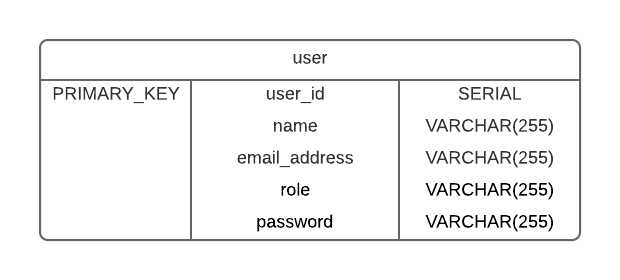
\includegraphics[scale=1.0]{erd_user}
\caption{The Entity Relationship Diagram of the user schema}
\end{figure}
\noindent
The user schema was created with simplicity in mind. The user authentication process is custom made. For the real product, CERN's own authentication process called OAuth will be used. Since this is temporary, it was decided to make this as simple as it was possible, since this is something that will disappear once the OAuth is working. The first iteration of the database scheme had the user bound to the subsystem, however, one of the requirements were changed to the fact that a shifter could be part of multiple subsystems. Therefore, this connections has been removed and a custom authentication system was created for the prototype. \\
This authentication system enables the user to login into the application. On the back end of the prototype, once the authentication has succeeded, a JWToken is sent to the front-end, mimicking the real system. To store the password safely into the database, the password was encrypt with the bcrypt[15] module. Bcrypt hashes the password with a salt, random data added to the hash, and then the prototype stores the password hashed into the database. The next diagram is the ERD of the log entry schema:
\begin{figure}[H]
\centering
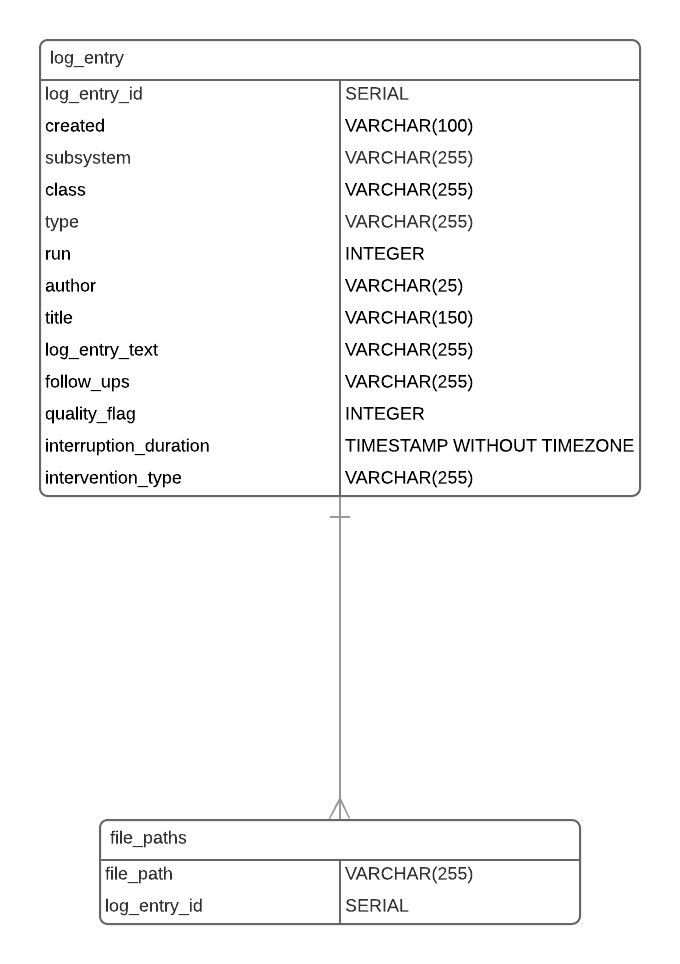
\includegraphics[scale=0.9]{erd_log_entry}
\caption{The Entity Relationship Diagram of the log entry schema}
\end{figure}
\noindent
The goal of designing the log entry schema was to keep it as simple as possible. One of the first iterations was a table for each kind of log entry (End of Shift report, On Call Intervention etc.), however, after receiving the feedback that the database design could combine the different types of log entries into one table, this iteration was chosen. With this design, it will be much easier to extend the log entry table where needed. The file paths are separated from the log entries, since with this design, it will be easier to add multiple files to one log entry. \\ 
During the development of the prototype, several frameworks and modules other than the WebUI framework have been used to create the prototype. These modules offered functionality that would either reduce the development time of the module or reduce the difficulty of the development. \\ \\
One module that was used, is mkdirp[16]. This module creates directories when the program is running. It is used when a file is uploaded on the server, so that the file is stored in a folder for every new log entry. Furthermore, the module PG[17] as an additional framework for setting up the database and executing queries was used. \\ Another module that has been used is the datetime[18] module. This module displays the current time. This is used whenever a log entry is added that this time is added to the log entry. Another module that has been used is the multer[19] module. This module was used to handle the file uploading. Instead of creating this functionality, it was easier to implement this module into the prototype. \\  
\\The final diagram is the class diagram of the prototype itself:
\begin{figure}[H]
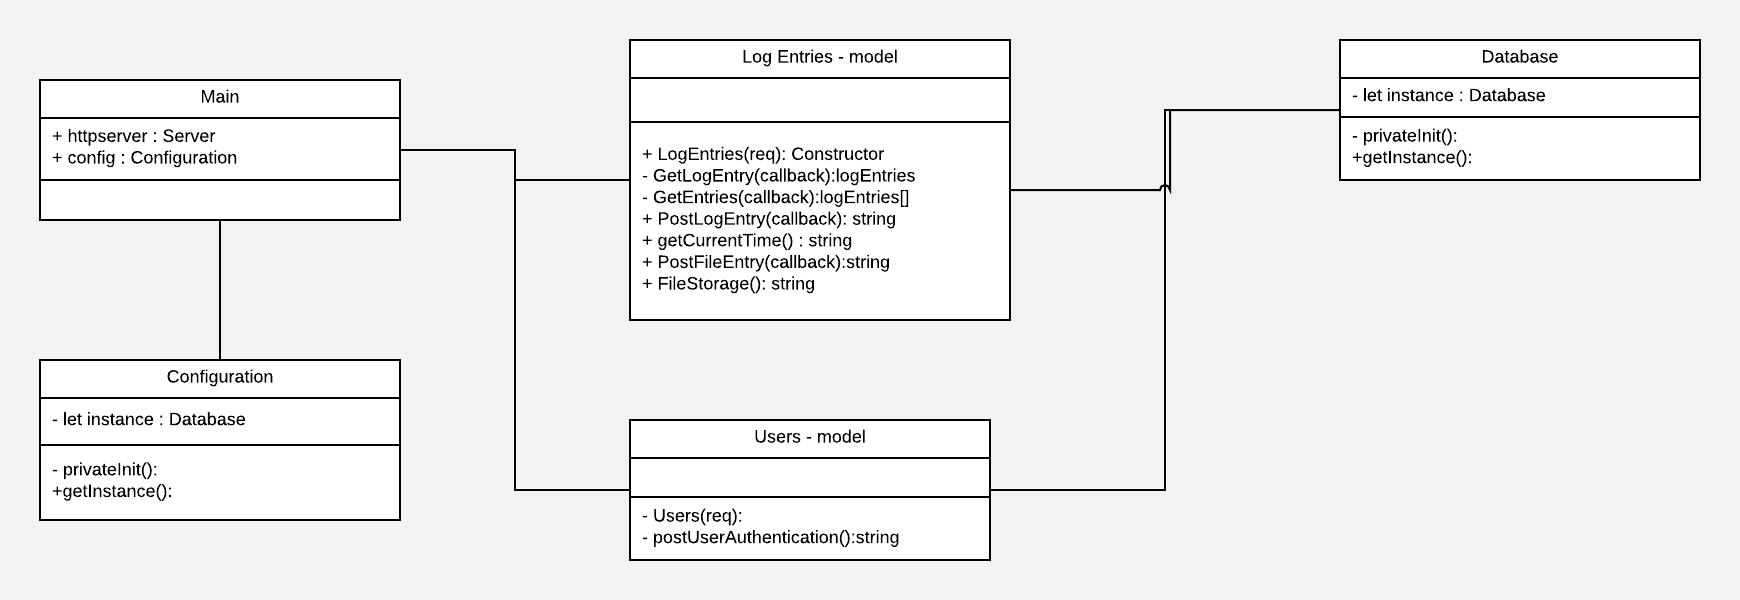
\includegraphics[scale=0.9]{class_diagram}
\caption{The class diagram of the prototype}
\end{figure}
\noindent
The class diagram contains the two chosen design patterns and the requirements that were chosen to be implemented into the prototype. The two design patterns are implemented, along with the required functionality that has been picked earlier.\\
As seen earlier, not all the requirements could be made into the prototype. These requirements will be displayed into an table with the reason why they could not be made into the prototype.
\newpage
\begin{longtable}{ | p{3cm} | p{7cm} | p{3cm}|}
\hline
Role & User Story & Reason \\ \hline
Subsystem expert & As a subsystem expert, I want to attach quality flags to runs so that physicists can use them while searching for good data sets for their analysis (Vasco Chibante Barroso).& Due to time constraints and the front end needed more time for polishing. \\ \hline
User & As a user, I want to search log entries by different criteria (e.g. title, content, author, creation date,(...) and have the results listed. & This user story is particually complete. It is possible to search log entries based upon run, author, subsystem and type of log entry. \\ \hline
Subsystem Run Coordinator &  As a subsystem responsible, I want to be notified by email (or other channels) of log entries which are related with my subsystem so that I can better follow-up activities without having to constantly visit the product, e.g. EOS report (Robert Munzer) (Vasco Chibante Barroso). & This was deemed to big due to the fact that a server must be made and an entire new piece of software must be added for the server. \\ \hline
System Run Coordinator & As subsystem run coordinator I may request to receive automatic emails concerning all Logbook entries that include the System I am working for (either without distinction or using special selection criteria s). The e-mail delivery address will probably be an e-group (single e-mail address <...>@cern.ch) (Roberto Divia). & This was deemed to big due to the fact that a server must be made and an entire new piece of software must be added for the server. \\ \hline
Run coordinator, S.R.C. and Administrator &  As run coordinator, S.R.C. or Admin, I must be able to move collaborators to and out of subsystem teams. These action may be conflict the information stored in SAMS (Roberto Divia). & The authentication software was not available on time to be used for the prototype. \\ \hline
\end{longtable}
The design patterns Singleton and MVC could be implemented into the prototype. The view part of the MVC design pattern is not implemented into the prototype. The reason for this was, that the front-end could not work with the way the data that came out of the view. This was done late in the development process and would mean significant changes in the code from the front-end. After discussing this with the front-end, this resulted into removing the view part. The singleton of the database can be found below: 
\newpage
\begin{lstlisting}[language=JavaScript, frame=single]
/*
 * Copyright (C) 2018 Amsterdam University of Applied Sciences (AUAS)
 *
 * This software is distributed under the therms of the
 * GNU General Public Licence version 3 (GPL) version 3,
 * copied verbatim in the file "LICENSE"
 *
 */

const Database = (() => {
  'use strict';
  let instance;

  /**
   * Initializes the database
   * @return {database} Returns the database singleton
   */
  function privateInit() {
    const pg = require('pg');
    const {Log} = require('@aliceo2/web-ui');
    const Config = require('./configuration_files/Config.js').Config;
    const config = Config.getInstance();
    const client = new pg.Client(config.getDatabaseConfiguration());
    client.connect()
      .then(() => Log.debug('Database connected.'))
      .catch((e) => Log.error(e.stack));

    return {
      getClient: function() {
        return client;
      }
    };
  }
  return {
    getInstance: () => {
      if (!instance) {
        instance = privateInit();
      }
      return instance;
    }
  };
})();
module.exports = {Database};

\end{lstlisting} 

Combining different technologies and frameworks, design patterns and the list of chosen requirements, a prototype could be made. Not all requirements and a part of the design pattern could be implemented in the prototype. This had to do either with time constraints or the use of special technology which would take too much time to complete.
\newpage
\subsection{Test cases}
Once the prototype was created, test cases were needed to verify that the prototype was actually working. After creating an test case template, different scenario's were chosen to create tests for. With the test cases, it was possible to create automated tests with the help of Mocha[14]. Mocha is a tool to create different kinds of tests like unit tests(small, simple tests to test a small piece of code) and integration tests(larger and more complex tests to test entire features). These test cases can be found as an attachment under section one point four, due to the amount of test cases created. Two test cases along with code and an explanation will be shown. The tests have been divided into two parts. \\ \\
The first part of the tests is testing the controller side, the end points, of the prototype, testing if parameters are passed successfully and testing if the token works as it should work. The second part of the tests is about interacting with the database. The models are verified that they are working. Furthermore, the interactions with the database are being tested.  \\ \\
The first test case, a test about the end points, is shown below:
\subsubsection{Test case 3}
\textbf{System}:  ALICE Bookkeeping prototype \\
\textbf{Test Case Name}:  Get non existing log entry
\textbf{Subsystem}:  Http-requests
\textbf{Designed by}:  Frederick van der Meulen\\
\textbf{Design date}: 30/05/2018 \\
\textbf{Short description}: The user tries to retrieve a log entry that does not exist. \\

Pre-conditions: 
\begin{enumerate}
\item The user is logged into the application
\end{enumerate}

\begin{longtable}{ | p{0.8cm} | p{4.5cm} | p{6cm}  | p{1.5cm} |}
\hline
Step & Action & Expected System Response & Pass/Fails  \\ \hline
1 & The user fills into the search bar of the web browser the URL to the non existing log entry. & The system tries to process the request, but fails because the log entry does not exist &  \\ \hline
2 & The user sees an error message stating that the log entry does not exist & The system sends the error message to the client as a result of not finding the log entry. &  \\ \hline
\end{longtable}
\newpage
This test case is about the scenario of whenever a user tries to retrieve a log entry that does not exist. It can happen that the user wants to see a log entry quickly, but makes a small mistake. If no error message is given, the user will not be notified about the missing log entry or the system shuts down, because the system can't complete the request. \\ 
For this test, the following code was used to make sure that the test case is verified :
\begin{lstlisting}[language=JavaScript, frame=single]
it('should return a json with an error message that the log entry does not exist', (done) => {
  request('http://localhost:' + config.getServerConfiguration().port
    + '/api/1111?token=' + token, (error, res, body) => {
    const parsedBody = JSON.parse(body);
    assert.strictEqual(res.statusCode, 404);
    assert.strictEqual(parsedBody[0].error_message, 'The entry could not be retrieved');
    });
  done();
});

\end{lstlisting}

The second test case is about testing the possibility of creating a log entry. This test case interacts with the database, as described earlier. To prevent that the production database is being tempered with, a test database has been created. This test database is identical to the regular one, but without the risk of losing data that has been stored on the regular database. The test case can be found below:

\subsubsection{Test case 8}
\textbf{System}:  ALICE Bookkeeping prototype \\
\textbf{Test Case Name}:  Post log entry
\textbf{Subsystem}:  Database-request
\textbf{Designed by}:  Frederick van der Meulen\\
\textbf{Design date}: 30/05/2018 \\
\textbf{Short description}: The user creates a log entry. \\

Pre-conditions: 
\begin{enumerate}
\item The user is logged into the application.
\end{enumerate}


\begin{longtable}{ | p{0.8cm} | p{4.5cm} | p{6cm}  | p{1.5cm} |}
\hline
Step & Action & Expected System Response & Pass/Fails  \\ \hline
1 & The user fills in all the fields that holds information for the log entry and presses submit. & The system receives the request and starts to process it. &  \\ \hline
2 & The user receives an message that the log entry is successfully posted & The systems sees that all the information is correct and adds the log entry to the database. &  \\ \hline
\end{longtable}

This test is about creating log entries. Since this is one of the core features of the application, it is important that this feature keeps working, no matter which circumstances the software is being developed. 
Since this test is more complex, due to testing the database, the following code snippet has been created to verify the test case:

\begin{lstlisting}[language=JavaScript, frame=single]
mockPostLogEntryRequest = mocks.createRequest({
      method: 'POST',
      url: '/api/run/:runId/:subsystem/:class/:user',
      params: {
        runId: 2,
        subsystem: 'WTL',
        class: 'MACHINE',
        user: 'AlfredFutterkiste'
      },
      body: {
        type: 'EOS',
        title: 'Test',
        log_entry_text: 'Testing the tests'
      }
    });
    
  it('should be able to add a log entry into the system', (done) => {
    const postEntry = new logEntry.LogEntries(mockPostLogEntryRequest);
    postEntry.postDataEntry((result) => {
      expect(result[0]).to.not.be.null;
      expect(result[0]).to.have.a.property('log_entry_id');
    }).catch((ex) => log.error(ex));
    done();
  });


\end{lstlisting}


For some test cases, it was discovered that the code was not complete enough. This means that the test could not be made, since the code for the test did not exist. These lines of code were added to complete the test cases. \\
Some test cases could be combined into one test. For instance, the test case regarding logging into the system and the test case about that a token should always be provided are combined together into one programmed test. \\
There are two test cases that could not be verified. The first test case was about different node versions. This is easy to do manually by creating a new Virtual Machine and put a different node version there, but programmatically it was not doable. This was verified manually on a different virtual machine. \\ 
The second test case was about the configurations file missing. This test case could be possible to implement as a test, however, due to time constraints this test case could not be implemented as a test. This test case is verified manually.\\ \\

The test cases were created based upon a list of possible scenarios that were created. Based on the test cases, tests were programmed to verify the test cases. The result is that the tests have verified that the prototype is working as intended. 

\newpage
\section{Conclusion}
The research question of the thesis was: \\ \\
\textit{Which requirements can be implemented into the logbook system for ALICE?} \\

Once the unknown requirements were made clear with interviewing a former shifter, the requirements could be analysed and resulted into a list of prioritized requirements. The list of prioritzed  requirements has been discussed with the front end, which resulted in a smaller list of requirements, which was shrunk down after discussions with Software for Science. \\ The final list of requirements has been used to develop the prototype of the bookkeeping system. During the development of the prototype, several frameworks, modules and design patterns were used to either improve the quality of the prototype or to ease the development of the prototype. Not all requirements could be implemented into the prototype. These requirements had a scope that was to big or could not be made into the prototype due to the limited amount of time available or could not be implemented due to missing software from CERN. Finally, test cases were created with the prototype that were implemented as tests to verify that the prototype was working as intended. \\ \\
The requirements that were implemented into the prototype were requirements about creating log entries, uploading files to log entries and about a user login. 
%The requirements that were implemented were requirements about creating log entries. These requirements were chosen based upon analysing which requirements matched, or came close to matching, the predefined criteria by CERN and Software for Science. \\
%With the analysed requirements, a list of requirements that will be implemented into the prototype was made based upon discussions with the frontend and Software for Science. \\ \\ 
%The requirements that could not be made into the prototype were requirements that would be too big to implement and requirements that could not be made due to time constraints. During the development of the prototype, frameworks, modules and design patterns have been used to improve the quality of the prototype. \\
%When the prototype was completed, test cases were created to verify that the prototype was working. These test cases were implemented as either unit or integration tests in the code. 

\newpage
\section{Recommendations}
During the development of the bookkeeping prototype, the use of frameworks / modules were sometimes questioned, alongside other possible issues were encountered. Instead of adding these issues with the results , these issues with recommendations on how to prevent them in the future can be found in this chapter. \\ 


\subsection{Requirement Analysis}
The requirement document that was created consisted of many unknown terms, like DAQ, End of Shift report etcetera. For the actual development of the bookkeeping system, it is useful to have either a glossary that describes all these terms or to clarify these requirements at the start of the development. Otherwise, wrong assumptions can be made regarding the implementation of unclear features. \\
With the analysis, a lot of duplicate requirements were found. The recommendation is to make sure that these duplicate requirements are either removed, or ordered, otherwise, the same requirement could get a different priority. \\


\subsection{Consequences}
Make sure that the goals that are being set are realistic. There is always a delay with developing software that must be taken in account. This can be prevented with applying the Scrum method. For instance, with the stand-ups, it is easier to see where something goes wrong and take the appropriate actions where necessary. The retrospectives can make sure that all the issues that were encountered are communicated towards the project leaders and solutions are created for the issues. It would help as well if there was a look at the Sprint backlog once in a while to check the progress of the team so that it will be easier to improve that. \\
Another thing to take note is that future developers should ask early on for help whenever something like a additional server is needed. This was not done when the email server was needed, and therefore, user stories related to the email could not be completed. This would be a shame if this would happen with the actual development.

\newpage
\subsection{Prototype}
When the prototype was created, several different kinds of frameworks and technologies were used. One of these technologies was the WebUI backend framework from CERN. This framework consists of many additional modules, from which only two were used: the logging and the authentication with the JsonWebTokens. The JsonWebtokens was difficult to work with at the back end, since it was hard to retrieve the token due to the fact that CERN did not had their authentication method available for use. The logging module was nice, but offers little additional features above other logging modules. Therefore, it is recommended to discuss whenever WebUI would be useful for the actual development of the bookkeeping system. \\
When the prototype was being developed, modules and other frameworks have been used. These frameworks and modules reduced the development time of the prototype. It is recommended to use these modules and frameworks, in particular the mkdirp module for organizing the uploaded files for each log entries. Be aware of the duration of support of these modules and frameworks, since it could be a problem when the support suddenly drops while the bookkeeping system is in production. \\


\subsection{Test cases}
It is recommended to create test cases and make sure that the developers that will work on the actual product will create test cases with every sprint. However, keep in mind that the execution of the test cases with programmed tests take a lot of time to realise if the test fits the test case. \\
The testing framework, Mocha, was helpful with making the tests. It is possible to order the tests in different groups. For the prototype, the tests were divided in database tests and test with the end points. Be sure that the tests are divided, so that it will be easier to see which test succeed and which test fail in what category.

\newpage

\section{Glossary}
This section of the report will explain terms that will be used during the report. 
\begin{enumerate}
\item Http-request = Hypertext Transfer Protocol is an application protocol used to send and retrieve information over the internet. An request is whenever the client asks to the website to do an task.
\item Client = The computer that the users uses to e.g. look at websites.
\item Server = A computer or device that provides functionality to other clients.
\item JsonWebToken = JSON Web Token is an open standard that defines a compact and self-contained way for securely transmitting information between parties as a JSON object.
\item Continues integrated testing = Testing the product where multiple developers work in the same repository.
\end{enumerate}


\newpage
\section{Bibliography}
(1): Fast, unopinionated, minimalist web framework for Node.js. (n.d.). Retrieved May 16, 2018, from https://expressjs.com \\ 
(2): The World's Most Advanced open source relational database. (n.d.). Retrieved May 16, 2018, from https://www.postgresql.org/ \\
(3): Ansible, (n.d), Retrieved 14 June 2018, from https://www.ansible.com/
(4): The fun, simple, flexible JavaScript test framework. (n.d.). Retrieved May 16, 2018, from https://mochajs.org/ \\
(5): Sublime text 3. (n.d.). Retrieved May 16, 2018, from https://www.sublimetext.com/3 \\
(6): Schwaber, K. (1997). SCRUM Development Process. Business Object Design and Implementation, 117-134. doi:10.1007/978-1-4471-0947-1 11\\ 
(7): Git. (n.d.). Retrieved May 16, 2018, from https://git-scm.com/ \\
(8): Buede, Dennis M.; Miller, William D. (2016). The Engineering Design of Systems. Wiley. \\
(9): Achimugu, P., Selamat, A., Ibrahim, R., and Mahrin, M. N. (2014). A systematic literature review of software requirements prioritization research. Information and Software Technology, 56(6), 568-585. doi:10.1016/j.infsof.2014.02.001 \\
(10): Karlsson, J., Wohlin, C., and Regnell, B. (1998). An evaluation of methods for prioritizing software requirements. Information and Software Technology, 39(14-15), 939-947. doi:10.1016/s0950-5849(97)00053-0 \\
(11): Teitsma, M., Dr. (2018, March 29). Requirements Bookkeeping application ALICE [Pdf]. \\
(12): Online Diagram Software and Visual Solution. (2018, May 01). Retrieved May 16, 2018, from https://www.lucidchart.com/ \\
(13): Kaner, Cem. Testing Computer Software. Wiley, 2012.
 Retrieved June 20, 2019 \\
(14): Mocha, (n.d.) Retrieved June 27, 2018, from https://mochajs.org/ \\
(15): Osmani, A. (2013). Learning JavaScript design patterns. Sebastopol, CA: OReilly Media. \\
(16): Foundation, N. (n.d.). Retrieved August 16, 2018, from https://nodejs.org/en/ \\
(17): The Scrum Guide™. (n.d.). Retrieved August 16, 2018, from https://www.scrumguides.org/scrum-guide.html \\
(18): Node-datetime. (n.d.). Retrieved August 16, 2018, from https://www.npmjs.com/package/node-datetime \\
(19): Multer. (n.d.). Retrieved August 16, 2018, from https://www.npmjs.com/package/multer

\newpage

\section{Attachments}
\setcounter{section}{1}
\subsection{Interview transscript}

\includepdf[pages=-]{Transscript.pdf}


\subsection{Entries}
\begin{longtable}{ | p{2cm} | p{8cm} | p{1.5cm} | l |}
\hline
Role & User Story & Piority & Time \\ \hline
Administrator &  Only administrator may be given the possibility to remove log entries
(and I am not even sure about this) (Roberto Divia). & 1 & 8 \\ \hline
\end{longtable}

\subsubsection{Forum}
\begin{longtable}{ | p{2cm} | p{8cm} | p{1.5cm} | l |}
\hline
Role & User Story & Piority & Time \\ \hline
User &  As a user, I want to reply to existing log messages so that a conversation stays in a well-defined thread & 4 & 20 \\ \hline
User &  People can create issues (Pierre vanden Vyvre) & 1 & 13 \\ \hline


\end{longtable}

\subsubsection{View}
\begin{longtable}{ | p{2cm} | p{8cm} | p{1.5cm} | l |}
\hline
Role & User Story & Piority & Time \\ \hline
User &  As a user, I want to list log entries in a summary view so that I can
get an overview of what happened in a given period. & 8 & 8 \\ \hline
User &  As a user, I want to list log entries in a detailed view so that I can read them one after the other. & 8 & 2 \\ \hline
User &  As a user, I want to browse through all the available metadata associated with a given run to understand on which conditions the run was made. & 4 & 5 \\ \hline
Shifter & . As a shifter I want to view log entries. & 9 & 5 \\ \hline
Shifter &  As a shifter I want to view on call interventions. & 4 & 5 \\ \hline
Run coördinator &  As run coordinator, I want to specify acquisition targets for certain
time periods and check how far we are in achieving them so that I can
keep track of progress (Vasco Chibante Barroso). & 5 & 8 \\ \hline
SRC &  As System Run Coordinator I need ways to interrogate all the runs where the System I am responsible for participated and to get access to individual run entries and to summary statistics (Roberto Divia). & 2 & 13 \\ \hline
\end{longtable}

\newpage
\subsubsection{Search}
\begin{longtable}{ | p{2cm} | p{8cm} | p{1.5cm} | l |}
\hline
Role & User Story & Piority & Time \\ \hline
User & As a user, I want to search log entries by different criteria (e.g. title, content, author, creation date,(...) and have the results listed. & 9 & 8 \\ \hline
User &  As a user, I want to list all runs that match a given criteria to create my own run set. & 8 & 8 \\ \hline
User & As ALICE collaborator I need to check the details of any run: EOR
reason, statistics, log entries (Roberto Divia). & 6 & 5 \\ \hline
Run coördinator &  As run coördinator I may have to cross-reference log entries (e.g. by URL, by unique Reference ID, or by run number) (Roberto Divia). & 4 & 8 \\ \hline
Run coördinator, Shifter, SRC and STC &  As run coördinator, Shifter, SRC and STC I may need to cross reference log entries or other logbook fields (e.g. run numbers, fill numbers etc...) with whatever issue tracking system will be used by the ALICE collaboration (today: Jira). This association may also be done automatically by daemons(e.g. what is done today for EOR reasons and Jira tickets) (Roberto
Divia). & 2 & 8 \\ \hline
Subsystem expert & As a subsystem expert, I want to store custom fields that are only
relevant to my subsystem so that I can correlate them with the rest
of the metadata repository (e.g. ‘fetch all runs with configuration X
where this happened to my detector’) (Vasco Chibante Barroso). & 1 & 4 \\ \hline
ECS / DAQ and SRC &  As ECS/DAQ System Run Coordinator I need a way to access information of runs matching a selection criteria I specify (timestamps, run numbers, run types, included detectors etc...). Navigation between runs must be easy and quick. The target is to check the global runs
(production and tests) for quality and errors (Roberto Divia). & 2 & 8 \\ \hline
SRC and System Team Member & As subsystem run coördinator I may have to cross-reference log entries
(e.g. by URL, by unique Reference ID, or by run number) (Roberto Divia). & 4 & 5 \\ \hline
CERN Administrator Officer &  As CERN administration officer I need to check all the on-call intervention records issued by CERN personnel (use case to be cross-checked
with EP-AID-DA management) (Roberto Divia). & 1 & 13 \\ \hline
Developer & As a developer, I want to programmatically fetch log entries that
match a given criteria so that I can build custom logic or applications based on existing data (Vasco Chibante Barroso). & 1 & 8 \\ \hline


\end{longtable}

\subsubsection{Creation}
\begin{longtable}{ | p{2cm} | p{8cm} | p{1.5cm} | l |}
\hline
Role & User Story & Piority & Time \\ \hline
User &  As a user, I want to have a smart editor to create my log entries
(WYSIWYG or Markup) and be able to use smart text so that messages look nice (e.g. links, code, . ..)& 4 & 8 \\ \hline
User &  As a user, I want to be able to save search criteria for later use so that I don’t lose time defining them at each visit. & 1 & 8 \\ \hline
Shifter &  A shifter makes an entry into the database consisting of several items. Each entry records the following items: time of creation,which class the creator originates: human, type of entry, general, EOS, DCS, number of run, author of the entry, title of the entry, log entry, follow ups, files and actions & 9 & 8 \\ \hline
Shifter &  As a shifter I want to be able to create log entries. & 9 & 8 \\ \hline
Shifter & As shifter I have to create log entries concerning any system (alone or in combination) (Roberto Divia). & 8 & 5 \\ \hline
Run coördinator & As run coördinator I have to create Logbook entries that cover almost all the Systems (e.g. global announcements or minutes) (Roberto Divia). & 1 & 8 \\ \hline
Run coördinator, SRC and STC & As run coördinator, subsystem run coördinator, system team member I have to create log entries concerning any system (alone or in combination) (Roberto Divia). & 4 & 8 \\ \hline
\newpage
\hline
On Call Expert & A person who is called for a specific intervention makes an entry into the log system consisting of the following items; time of creation, author, type of intervention;remote, onsite, title of entry, log entry & 2 & 8 \\ \hline
Gas Technician & As a gas technician I want to create log entries when I delivered gas
and other substances at Point 2. & 4 & 3 \\ \hline
Observer &  As an observer I want to be able to look at the bookkeeping without
the chance of adding or manipulating data. & 1 & 5 \\ \hline 
\end{longtable}

\subsubsection{Files}
\begin{longtable}{ | p{2cm} | p{8cm} | p{1.5cm} | l |}
\hline
Role & User Story & Piority & Time \\ \hline
User &  As a user, I want to attach files to log entries so that I can add additional non-textual information & 9 & 8 \\ \hline
Run coördinator, SRC, STC and Shifter& As run coördinator, SRC, STC or as Shifter, I may need to attach files to log entries. These files may contain text or binary information (PNGs, JPGs etc...) (Roberto Divia). & 8 & 8 \\ \hline

\end{longtable}
\newpage
\subsubsection{Flags}
\begin{longtable}{ | p{2cm} | p{8cm} | p{1.5cm} | l |}
\hline
Role & User Story & Piority & Time \\ \hline
Run coördinator and Administrator &  As run coördinator or administrator, I need to be able to update the logbook information for what concerns subsystems, in particular the run quality flag and the EOR reason(s). The question arises if subsystem run coördinators can update information associated to other systems (e.g. EOR
reasons) as it is the case today (Roberto Divia). & 2 & 8 \\ \hline
Subsystem expert & As a subsystem expert, I want to attach quality flags to runs so that
physicists can use them while searching for good data sets for their analysis (Vasco Chibante Barroso). & 8 & 8 \\ \hline
\end{longtable}

\subsubsection{Data Extraction}
\begin{longtable}{ | p{2cm} | p{8cm} | p{1.5cm} | l |}
\hline
Role & User Story & Piority & Time \\ \hline
Detector Expert & As a detector expert I would like be able to extract run/fill information in a format, which allows easier analysis than txt files, e.g. root-files to be able to do specific statistical analysis (Robert Munzer). & 1 & 13 \\ \hline
SRC &  As subsystem run coördinator I need to be able to update the logbook information for what concerns my system and other systems, in particular the run quality flag and the EOR reason(s). The question arises if subsystem run coördinators can update information associated to other systems (e.g. EOR reasons) as it is the case today (Roberto Divia). & 1 & 8 \\ \hline

\end{longtable}
\newpage

\subsection{Reports}
\begin{longtable}{ | p{2cm} | p{8cm} | p{1.5cm} | l |}
\hline
Role & User Story & Piority & Time \\ \hline
ALICE collaborator &  As ALICE collaborator I have to create statistics reports such as number of runs, quantity of data, number of events, summaries by trigger
classes etc... These reports will use selection criterias I will specify such as time spans, active systems (e.g. only the runs including my particular system), run type etc... & 1 & 20 \\ \hline
Shifter &  As a shifter, I want to have templates that prefill most of my end-of-shift reports from the available metadata so that I don’t need to fill inmyself what the system already knows (Vasco Chibante Barroso). & 2 & 13 \\ \hline
Shifter &  As a Shifter, I would like to have templates that automatically compile and format the data available in the system in order to write my end of shift report in a fast and uniform way. Currently in the ALICE logbook, I don’t like that I need to compile all the information myself and that
not all shifters use the same structure (Vasco Chibante Barroso). & 2 & 13 \\ \hline
Run coördinator &  As run coördinator, I want shifters to use templates so that it is easier
and faster to read them (Vasco Chibante Barroso). & 1 & 13 \\ \hline
Subsystem Run Coördinator & As a SRC I would like to be able to create my own detector specific templates for example On-Call interventions. In this case I can specify the relevant information which are required from the OnCall shifter for different kind of “standard” events (Robert Munzer). & 8 & 20 \\ \hline
\end{longtable}
\newpage
\subsection{Email}
\begin{longtable}{ | p{2cm} | p{8cm} | p{1.5cm} | l |}
\hline
Role & User Story & Piority & Time \\ \hline
ALICE member & As an ALICE member, I would like to receive via email a global summary of each LHC Fill in order to follow ALICE operations without visiting the bookkeeping tools. Currently in the ALICE logbook, I like that I receive via email a document with info on efficiency and EOR Reasons and that on the body of the email there is a summary for
each fill (Vasco Chibante Barroso). & 8 & 20 \\ \hline
Run coördinator & As run coördinator I may request to receive automatic e-mails concerning all Logbook entries that include all systems (either without distinction or using special selection criterias). The e-mail delivery address will probably be an e-group (single e-mail address <...>@cern.ch)(Roberto Divia). & 6 & 13 \\ \hline
Subsystem Run Coördinator &  As a subsystem responsible, I want to be notified by email (or other
channels) of log entries which are related with my subsystem so that I can better follow-up activities without having to constantly visit the product, e.g. EOS report (Robert Munzer) (Vasco Chibante Barroso). & 8 & 13 \\ \hline
SRC & As subsystem run coördinator I may request to receive automatic emails concerning all Logbook entries that include the System I am working for (either without distinction or using special selection criterias). The e-mail delivery address will probably be an e-group (single e-mail address <...>@cern.ch) (Roberto Divia). & 8 & 13 \\ \hline
SRC & . The subsystem coördinator wants to be reported when something is going on with his system. He should not have to take action for himself to find out things (Robert Helmut Munzer). & 6 & 13 \\ \hline

\end{longtable}
\newpage
\subsection{Roles and Authentication}
\begin{longtable}{ | p{2cm} | p{8cm} | p{1.5cm} | l |}
\hline
Role & User Story & Piority & Time \\ \hline
User & As a user, I want to be able to login with my CERN credentials to avoid having to remember a new set of credentials. This should be done by using the CERN authentication method. & 9 & 13 \\ \hline
Run coördinator, SRC and Administrator &  As run coördinator, SRC or Admin, I must be able to move collaborators to and out of subsystem teams. These action may be conflict the information stored in SAMS (Roberto Divia). & 9 & 13 \\ \hline
Run coördinator, SRC, Administrator & As run coördinator, SRC or Administrator, access to Logbook actions restricted to my role should be granted without external interventions and for the time span of my duties (e.g. for shifters the shifts before and after mine, plus my own shift) (Roberto Divia). &4 & 8\\ \hline
Run coördinator and SRC &  As run coördinator or SRC I need to give ALICE collaborators write or read-only access to the logbook. These rights will be superseeded by equivalent rights given according to the function of the user (e.g. a ALICE collaborator with read-only access will be given write access during the time of his/her duties as a shifter, subsystem run coördinator or system team member) (Roberto Divia).&6&13 \\ \hline
\end{longtable}
\newpage
\subsection{View with Dash boards}
\begin{longtable}{ | p{2cm} | p{8cm} | p{1.5cm} | l |}
\hline
Role & User Story & Piority & Time \\ \hline
User &  As a user, I want to see in a dashboard the metadata associated with
an LHC Fill so that I can have a global image of what happened during that LHC Fill. & 2 & 13 \\ \hline
User &  As a user, I want to be able to customize dashboards so that I only see the fields relevant to me. & 1 & 13 \\ \hline
User &  As ALICE collaborator I may have to open multiple GUIs with independent selection criterias (e.g. one browser window for day-to-day work and a second browser window for statistics) (Roberto Divia). & 1 & 20 \\ \hline
ALICE collaborator &  As ALICE collaborator I need to be able to access the Logbook on a run-per-run summary view (possibly using a selection criteria I specify) and on a log entry by log entry view (possibly using a selection criteria
I specify) (Roberto Divia). & 1 & 13 \\ \hline
Shifter & As a shifter I want to view data about calibration of the detector. & 4 & 5 \\ \hline
Shifter & As a shifter I want to be able to have a big screen view. & 2 & 3 \\ \hline
Shifter & As a shifter I want to view data about the fill. & 1 & 5\\ \hline
Physics Community & The Physics Board has several needs or questions:
1. To make the planning possible an overview of storage and processing
power (CPU) is needed.
2. The use of resources per user to run jobs could be more detailed.
3. How much PB is available on disk for storage.
4. For MC-storage a fine grained but lacks an overview.
5. When I want to clean up, where do I have to look?
6. MC production requests.
7. Usage statistics (which data is popular?).
8. Sort out why a train takes a specific time to process. & 1 & 13\\ \hline
Physics Community & Most data is replicated because a lot of people use the data.
There are two views from the Physics Board:
• clean up, to know what could be cleaned up
• planning, when can this MC be run?
& 1 & 13 \\ \hline
Adminis-trator & As an administrator, I want to have a dashboard that gives me log-
entry related analytics so that I follow the evolution of the repository
(Vasco Chibante Barroso). & 1 & 13 \\ \hline

\end{longtable}

\subsection{Statistics}
\begin{longtable}{ | p{2cm} | p{8cm} | p{1.5cm} | l |}
\hline
Role & User Story & Piority & Time \\ \hline
Shifter &  As a shifter I want to view some statistics of runs and other stuff. & 1 & 8 \\ \hline
Run coördinator &  As run coördinator I need to gather statistics on the runs selected by using custom rules (timestamps, run numbers, run types, included detectors etc...). These statistics will include EOR reasons, per-detector and per-system summaries, error recovery (PARs) rates etc.(Roberto Divia) & 1 & 13 \\ \hline
Physics Community &  Each week global and specific statistics about the system are needed
• CPU usage
• data storage
• etc. & 1 & 13 \\ \hline


\end{longtable}

\subsection{Run}
\begin{longtable}{ | p{2cm} | p{8cm} | p{1.5cm} | l |}
\hline
Role & User Story & Piority & Time \\ \hline
Run coördinator &  As run coördinator, I want to attach tags to runs so that I can then use them while searching (Vasco Chibante Barroso). & 4 & 8 \\ \hline
Run coördinator &  As run coördinator, I want to edit certain specialized fields associated to a run (e.g. EOR Reason) so that I correct wrong information inserted by the O 2 software (Vasco Chibante Barroso). & 1 & 5 \\ \hline
Developer &  As a developer, I want to programmatically fetch runs that match a
given criteria so that I can build custom logic or applications based on
existing data (Vasco Chibante Barroso). & 1 & 8 \\ \hline
\end{longtable}
\newpage
\subsection{Announcements}
\begin{longtable}{ | p{2cm} | p{8cm} | p{1.5cm} | l |}
\hline
Role & User Story & Piority & Time \\ \hline
Shifter &  As a shifter I want to view announcements. & 4 & 5 \\ \hline
Adminis-trator & System administrators can create an announcement. This announce-
ment consists of the following items: time of creation, validity, duration of interruption of the system, author, title of the entry, log entry & 2 & 8 \\ \hline
\end{longtable}

\subsection{Other}
\begin{longtable}{ | p{2cm} | p{8cm} | p{1.5cm} | l |}
\hline
Role & User Story & Piority & Time \\ \hline
Managet & As a manager I want to know whether all the relevant people are
involved with respect to an issue (Pierre vanden Vyvre). & 1 & 13 \\ \hline
Adminis-trator & As administrator I may request to replicate either selected portions
or all of the Logbook data to external sites and to provide adequate access tools to it (to facilitate read-only accesses) (Roberto Divia). & 1 & 20 \\ \hline
Adminis-trator & As an administrator I must be able to configure the system. & 1 & 13 \\ \hline


\end{longtable}



\subsection{Test case template}

\textbf{System}:  The name of the system \\
\textbf{Test Case Name}:  The name of the test case
\textbf{Subsystem}:  Which part of the system gets tested
\textbf{Designed by}:  Who designed this test\\
\textbf{Design date}: When was this test designed \\
\textbf{Short description}: Description of the test case \\

Pre-conditions: \\
\begin{enumerate}
\item What are the conditions the system needs to be before the test starts
\end{enumerate}

\begin{longtable}{ | p{0.8cm} | p{4.5cm} | p{6cm} | p{1.5cm} |}
\hline
Step & Action & Expected System Response & Pass/Fails  \\ \hline
1 & What does the user needs to do & How does the system responds to this & Is the test passed or failed with this step  \\ \hline

\end{longtable}

\subsection{The ideas}

\subsubsection{Requests}

\subsubsection{GET}
\begin{enumerate}
\item Get request successfully
\item Get non existing single log entry
\item Get duplicate single log entry
\item Get all entries but without any entries into system
\item Get file from single entry
\item Get file from single entry that has no file
\item Get file from single entry, but the file was corrupted
\item Get file from single entry, but the server connection fails
\end{enumerate}

\subsubsection{POST}
\begin{enumerate}
\item Post single log entry successfully
\item Post single log entry with values missing
\item Post single log entry when someone has just create a single entry
\item Attach file to log entry successfully
\item Attach file to log entry but the process gets corrupted
\item Attach file to log entry but the path doesn't match the actual location
\end{enumerate}

\subsubsection{Other requests}
\begin{enumerate}
\item Client wants to do a not supported request
\item Request with non existing token or a token created with third parties

\end{enumerate}

\subsubsection{Database}
\begin{enumerate}
\item Database connection fails during request
\item Database query fails to succeed 
\item The database can be upgraded to a different version 
\end{enumerate}



\subsubsection{Login}
\begin{enumerate}
\item Client logs into the application successfully
\item Client logs into the application but the password and email don't match
\item Client logs in, but the client doesn't receive a token
\item Client logs in and receive a token, but the token is of the wrong access level
\end{enumerate}

\subsubsection{Configurations}
\begin{enumerate}
\item The configuration file is missing
\item The configuration file is incomplete and certain features don't work any more
\item The configuration file that the users uses doesn't match the one that the back-end needs.
\item When there is an error in the system, the error gets logged into an log file.
\end{enumerate}

\subsubsection{Misbehaviour of client}
\begin{enumerate}
\item Client tries to perform a SQL injection
\item The file that is attached to a log entry is a virus
\item Client tries to perform an Http request for which the client doesn't have the rights for.
\item Client tries to change it's rights level within the application

\end{enumerate}

\subsubsection{Different versions}
\begin{enumerate}
\item A machine has a higher node version than the server
\item A machine has a lower node version than the server
\item The port that the server runs on is already used by another application
\item The port number is lower than one
\item The port number is higher than a million
\item The server can be upgraded to a different node version
\end{enumerate}

\subsection{Test cases}

\subsubsection{Test case 1}
\textbf{System}:  ALICE Bookkeeping prototype \\
\textbf{Test Case Name}:  Get corrupted file from system
\textbf{Subsystem}:  Http-requests
\textbf{Designed by}:  Frederick van der Meulen\\
\textbf{Design date}: 30/05/2018 \\
\textbf{Short description}: Get file from single entry, but the file was corrupted. The user needs to be notified of this corruption \\

Pre-conditions: \\
\begin{enumerate}
\item The user added a file to the log entry.
\item The file got corrupted during adding the file
\end{enumerate}

\begin{longtable}{ | p{0.8cm} | p{4.5cm} | p{6cm} | p{1.5cm} | p{1.5cm} |}
\hline
Step & Action & Expected System Response & Pass/Fails & Comment \\ \hline
1 & Click the log entry & The system shows the detailed log entry & & \\ \hline
2 & Click on the file that the user wants to download & The system receives the GET request & & \\ \hline
3 & Press download & The file is being downloaded by the client & & \\ \hline
\end{longtable}
\subsubsection{Test case 2}
\textbf{System}:   ALICE Bookkeeping prototype\\
\textbf{Test Case Name}:  POST corrupted file to log\\
\textbf{Subsystem}:  \\
\textbf{Designed by}:  Frederick van der Meulen\\
\textbf{Design date}:  31/05/2018\\
\textbf{Short description}: Attach file to log entry but the process gets corrupted \\

Pre-conditions: \\
\begin{enumerate}
\item The user has the rights to create a log entry
\item The user has created the file that the user wants to attach to the log entry
\end{enumerate}

\begin{longtable}{ | p{0.8cm} | p{4.5cm} | p{6cm} | p{1.5cm} | p{1.5cm} |}
\hline
Step & Action & Expected System Response & Pass/Fails & Comment \\ \hline
1 & Select the file for uploading & The system does nothing at the moment & & \\ \hline
2 & Press the send file button & The server receives the file, however, something in the process goes wrong. & & \\ \hline
3 & Receive a message that the file got corrupted & Instead of adding the file path to the database, a message that the file got corrupted gets added to the database. & & \\ \hline
\end{longtable}

\subsubsection{Test case 3}
\textbf{System}: ALICE Bookkeeping prototype\\
\textbf{Test Case Name}: Unauthorized request\\
\textbf{Subsystem}:  \\
\textbf{Designed by}: Frederick van der Meulen \\
\textbf{Design date}: 31/05/2018 \\
\textbf{Short description}: Client tries to perform an Http request for which the client doesn't have the rights for. In this example, a shifter will try to change the users in it's sub system. \\

Pre-conditions: \\
%\begin{enumerate}
%\end{enumerate}

\begin{longtable}{ | p{1cm} | p{3cm} | p{6cm} | p{1.5cm} | p{1.5cm} |}
\hline
Step & Action & Expected System Response & Pass/Fails & Comment \\ \hline
1 & Enter the subsystem run coordinator URL & The server receives the GET request from the client, but discovers that the access token is wrong & & \\ \hline
2 & Receive an error message that you're not allowed to do this. & The system returns an error message to the client & & \\ \hline 
\end{longtable}

\subsubsection{Test case 4}
\textbf{System}:  ALICE Bookkeeping prototype \\
\textbf{Test Case Name}:  Get non existing single log entry \\
\textbf{Subsystem}:  Http-requests \\
\textbf{Designed by}:  F.P. van der Meulen\\
\textbf{Design date}:  \\
\textbf{Short description}: The user tries to retrieve the details of a single log entry that does not exist. \\

Pre-conditions: \\
%\begin{enumerate}
%\end{enumerate}

\begin{longtable}{ | p{0.8cm} | p{4.5cm} | p{6cm} | p{1.5cm} |}
\hline
Step & Action & Expected System Response & Pass/Fails  \\ \hline
1 & The user fills into the search bar the log entry that does not exist yet. & The system tries to process the request, but fails because the entry does not exist &   \\ \hline
2 & The user sees an error message stating that the log entry does not exist. & The system sends the error message as the result of not finding the log entry. & Pass \\ \hline

\end{longtable}

\subsubsection{Test case 5}
\textbf{System}:  ALICE Bookkeeping prototype \\
\textbf{Test Case Name}:  Get duplicate single log entry \\
\textbf{Subsystem}:  Http-requests \\
\textbf{Designed by}:  F.P. van der Meulen\\
\textbf{Design date}:  \\
\textbf{Short description}: The user tries to retrieve the details of a single log entry , but two log entries have the same id. \\

Pre-conditions: \\
%\begin{enumerate}
%\end{enumerate}

\begin{longtable}{ | p{0.8cm} | p{4.5cm} | p{6cm} | p{1.5cm} |}
\hline
Step & Action & Expected System Response & Pass/Fails  \\ \hline
1 & The user fills into the search bar the log entry the user wants to see. & The system receives the request and processes it & Fails when the entry does not exist  \\ \hline
2 & The user sees an error message stating that the log entry does not exist. & The system sends the error message as the result of not finding the log entry. & Pass \\ \hline

\end{longtable}
\subsubsection{Test case 6}
\textbf{System}:  ALICE Bookkeeping prototype \\
\textbf{Test Case Name}:  Get all entries without any entries into the system. \\
\textbf{Subsystem}:  Http-requests \\
\textbf{Designed by}:  F.P. van der Meulen\\
\textbf{Design date}:  \\
\textbf{Short description}: The user tries to retrieve all the log entries, but there are no entries into the system. \\

Pre-conditions: \\
%\begin{enumerate}
%\end{enumerate}

\begin{longtable}{ | p{0.8cm} | p{4.5cm} | p{6cm} | p{1.5cm} |}
\hline
Step & Action & Expected System Response & Pass/Fails  \\ \hline
1 & The users presses the log entries button in the navbar & The system receives the request and processes it & Pass \\ \hline
2 & The user sees an empty screen. & The system sends an error message that are no entries into the system. & Pass \\ \hline

\end{longtable}
\subsubsection{Test case 7}
\textbf{System}:  ALICE Bookkeeping prototype \\
\textbf{Test Case Name}:  Get file from single entry. \\
\textbf{Subsystem}:  Http-requests \\
\textbf{Designed by}:  F.P. van der Meulen\\
\textbf{Design date}:  \\
\textbf{Short description}: The user tries to retrieve a file from a single log entry. \\

Pre-conditions: \\
\begin{enumerate}
\item The file storage process was successful
\item At least one file was added to one log entry
\end{enumerate}

\begin{longtable}{ | p{0.8cm} | p{4.5cm} | p{6cm} | p{1.5cm} |}
\hline
Step & Action & Expected System Response & Pass/Fails  \\ \hline
1 & The users fills in the url for downloading a file. & The system receives the request and processes it & Pass \\ \hline
2 & The user receives a prompt with downloading a file. & The system sends the file to the computer of the user & Pass
\end{longtable}
\subsubsection{Test case 8}
\textbf{System}:  ALICE Bookkeeping prototype \\
\textbf{Test Case Name}:  Get file from single entry that has no file. \\
\textbf{Subsystem}:  Http-requests \\
\textbf{Designed by}:  F.P. van der Meulen\\
\textbf{Design date}:  \\
\textbf{Short description}: The user tries to retrieve a file from a single log entry, but the entry does not have a file attached to it. \\

Pre-conditions: \\
%\begin{enumerate}
%\end{enumerate}

\begin{longtable}{ | p{0.8cm} | p{4.5cm} | p{6cm} | p{1.5cm} |}
\hline
Step & Action & Expected System Response & Pass/Fails  \\ \hline
1 & The users fills in the url for downloading a file. & The system receives the request and processes it & Pass \\ \hline
2 & The user receives an error that there is no file attached to the log entry. & The system sends the error message to the user that there is no file with the log entry & Pass
\end{longtable}

\subsubsection{Test case 9}
\textbf{System}:  ALICE Bookkeeping prototype \\
\textbf{Test Case Name}:  Post single log entry. \\
\textbf{Subsystem}:  Http-requests \\
\textbf{Designed by}:  F.P. van der Meulen\\
\textbf{Design date}:  \\
\textbf{Short description}: The user creates a log entry . \\

Pre-conditions: \\
%\begin{enumerate}
%\end{enumerate}

\begin{longtable}{ | p{0.8cm} | p{4.5cm} | p{6cm} | p{1.5cm} |}
\hline
Step & Action & Expected System Response & Pass/Fails  \\ \hline
1 & The users fills in all the fields that holds information for the log entry and presses submit & The system receives the request and starts to process it. & Pass \\ \hline
2 & The user receives an message that the log entry is successfully posted . & The system marks that all the information is correct and adds the log entry to the database. & Pass
\end{longtable}
\subsubsection{Test case 10}
\textbf{System}:  ALICE Bookkeeping prototype \\
\textbf{Test Case Name}:  Post single log entry with insufficient values. \\
\textbf{Subsystem}:  Http-requests \\
\textbf{Designed by}:  F.P. van der Meulen\\
\textbf{Design date}:  \\
\textbf{Short description}: The user tries creates a log entry, but mandatory fields are missing from the request. \\

Pre-conditions: \\
%\begin{enumerate}
%\end{enumerate}

\begin{longtable}{ | p{0.8cm} | p{4.5cm} | p{6cm} | p{1.5cm} |}
\hline
Step & Action & Expected System Response & Pass/Fails  \\ \hline
1 & The users fills in some fields, but not the mandatory fields and presses submit & The system receives the request and starts to process it. & Pass \\ \hline
2 & The user receives an message that the log entry is incomplete. & The system marks that some of the information is correct and sends an error message to the user. & Fail
\end{longtable}

\subsubsection{Test case 11}
\textbf{System}:  ALICE Bookkeeping prototype \\
\textbf{Test Case Name}:  Request without a token or a third party token. \\
\textbf{Subsystem}:  Http-requests \\
\textbf{Designed by}:  F.P. van der Meulen\\
\textbf{Design date}:  \\
\textbf{Short description}: The user tries to do a request without a token or a token that has been created with the help of third party tools \\

Pre-conditions: \\
%\begin{enumerate}
%\end{enumerate}

\begin{longtable}{ | p{0.8cm} | p{4.5cm} | p{6cm} | p{1.5cm} |}
\hline
Step & Action & Expected System Response & Pass/Fails  \\ \hline
1 & The users fills in a request and presses enter without a token or an invalid token & The system receives the request. &  \\ \hline
2 & The user receives an error stating that the token is invalid & The system does not recognize the token and sends an error message & Fail \\ \hline
\end{longtable}
\subsubsection{Test case 12}
\textbf{System}:  ALICE Bookkeeping prototype \\
\textbf{Test Case Name}:  Database connection fails during a request. \\
\textbf{Subsystem}:  Database \\
\textbf{Designed by}:  F.P. van der Meulen\\
\textbf{Design date}:  \\
\textbf{Short description}: When the user tries to do a request that involves the database, the database connection fails \\

Pre-conditions: \\
%\begin{enumerate}
%\end{enumerate}

\begin{longtable}{ | p{0.8cm} | p{4.5cm} | p{6cm} | p{1.5cm} |}
\hline
Step & Action & Expected System Response & Pass/Fails  \\ \hline
1 & The users fills in a request and presses enter  & The system receives the request. &  \\ \hline
2 & The user receives an error stating that the database connection timed out & The system can not connect to the database and the system sends an error message to the user. & Fail \\ \hline
\end{longtable}
\subsubsection{Test case 13}
\textbf{System}:  ALICE Bookkeeping prototype \\
\textbf{Test Case Name}:  Database query fails to succeed. \\
\textbf{Subsystem}:  Database \\
\textbf{Designed by}:  F.P. van der Meulen\\
\textbf{Design date}:  \\
\textbf{Short description}: The user tries to perform a request and the system sees that all the required values are correct, however, the query with the database fails for an unknown reason. \\

Pre-conditions: \\
%\begin{enumerate}
%\end{enumerate}

\begin{longtable}{ | p{0.8cm} | p{4.5cm} | p{6cm} | p{1.5cm} |}
\hline
Step & Action & Expected System Response & Pass/Fails  \\ \hline
1 & The users fills in a request and presses enter  & The system receives the request. &  \\ \hline
2 & The user receives an error stating that something went wrong with the database. & The system can connect to the database, but the query fails and therefore the system sends an error message to the user. & Fail \\ \hline
\end{longtable}

\subsubsection{Test case 14}
\textbf{System}:  ALICE Bookkeeping prototype \\
\textbf{Test Case Name}:  User logs into the application. \\
\textbf{Subsystem}:  Login \\
\textbf{Designed by}:  F.P. van der Meulen\\
\textbf{Design date}:  \\
\textbf{Short description}: The user is logging into the application. \\

Pre-conditions: \\
%\begin{enumerate}
%\end{enumerate}

\begin{longtable}{ | p{0.8cm} | p{4.5cm} | p{6cm} | p{1.5cm} |}
\hline
Step & Action & Expected System Response & Pass/Fails  \\ \hline
1 & The user fills in the email and password and presses enter. & The system receives the email and the password &  \\ \hline
2 & The user receives the token that belongs to the user. & The system retrieves the email address from the database, then verifies the corresponding password and creates an token based upon the information from the user and sends the token back to the front-end. & Pass \\ \hline
\end{longtable}

\subsubsection{Test case 15}
\textbf{System}:  ALICE Bookkeeping prototype \\
\textbf{Test Case Name}:  User logs into the application with not matching values. \\
\textbf{Subsystem}:  Login \\
\textbf{Designed by}:  F.P. van der Meulen\\
\textbf{Design date}:  \\
\textbf{Short description}: The user is logging into the application, but the password and the email address do not match with each other. \\

Pre-conditions: \\
%\begin{enumerate}
%\end{enumerate}

\begin{longtable}{ | p{0.8cm} | p{4.5cm} | p{6cm} | p{1.5cm} |}
\hline
Step & Action & Expected System Response & Pass/Fails  \\ \hline
1 & The user fills in an email address and some random characters and presses enter. & The system receives the email and the password &  \\ \hline
2 & The user receives an error message stating that either the email address or the password is not correct. & The system retrieves the email address from the database, then verifies the corresponding password. The email or the password do not match, so an error message is sent to the user.. & Fail \\ \hline
\end{longtable}
\subsubsection{Test case 16}
\textbf{System}:  ALICE Bookkeeping prototype \\
\textbf{Test Case Name}:  User logs into the application, but does not receive a token. \\
\textbf{Subsystem}:  Login \\
\textbf{Designed by}:  F.P. van der Meulen\\
\textbf{Design date}:  \\
\textbf{Short description}: The user is logging into the application, however, even though the verification is successful, the user does not receive a token. \\

Pre-conditions: \\
%\begin{enumerate}
%\end{enumerate}

\begin{longtable}{ | p{0.8cm} | p{4.5cm} | p{6cm} | p{1.5cm} |}
\hline
Step & Action & Expected System Response & Pass/Fails  \\ \hline
1 & The user fills in an email address and some random characters and presses enter. & The system receives the email and the password &  \\ \hline
2 & The user receives an error message stating that something went wrong and should try again & The system retrieves the email address from the database, then verifies the corresponding password.  The token could not be generated, and the system sends an error message to the user. & Fail \\ \hline
\end{longtable}

\subsubsection{Test case 17}
\textbf{System}:  ALICE Bookkeeping prototype \\
\textbf{Test Case Name}:  User logs into the application and receives a token, but the token is of the wrong access level \\
\textbf{Subsystem}:  Login \\
\textbf{Designed by}:  F.P. van der Meulen\\
\textbf{Design date}:  \\
\textbf{Short description}: The user is logging into the application, however, the user receives a token with the wrong access level. \\

Pre-conditions: \\
%\begin{enumerate}
%\end{enumerate}

\begin{longtable}{ | p{0.8cm} | p{4.5cm} | p{6cm} | p{1.5cm} |}
\hline
Step & Action & Expected System Response & Pass/Fails  \\ \hline
1 & The user fills in an email address and some random characters and presses enter. & The system receives the email and the password &  \\ \hline
2 & The user receives an error message stating that something went wrong and should try again & The system retrieves the email address from the database, then verifies the corresponding password.  The token is generated, but the access level is placed wrong within the token. The system regonizes the access level and sends an error to the user. & Fail \\ \hline
\end{longtable}

\subsubsection{Test case 18}
\textbf{System}:  ALICE Bookkeeping prototype \\
\textbf{Test Case Name}:  The configuration file is missing \\
\textbf{Subsystem}:  Configurations \\
\textbf{Designed by}:  F.P. van der Meulen\\
\textbf{Design date}:  \\
\textbf{Short description}: The user starts the webserver, however, there is no configuration file. \\

Pre-conditions: \\
%\begin{enumerate}
%\end{enumerate}

\begin{longtable}{ | p{0.8cm} | p{4.5cm} | p{6cm} | p{1.5cm} |}
\hline
Step & Action & Expected System Response & Pass/Fails  \\ \hline
1 & The user fills in the command to start the web server. & The system is starting up. &  \\ \hline
2 & The user receives an error message that the configuration file is missing. & The system can not find the configuration file and displays an error message & fail\\ \hline
 
\end{longtable}

\subsubsection{Test case 19}
\textbf{System}:  ALICE Bookkeeping prototype \\
\textbf{Test Case Name}:  The configuration file is incomplete \\
\textbf{Subsystem}:  Configurations \\
\textbf{Designed by}:  F.P. van der Meulen\\
\textbf{Design date}:  \\
\textbf{Short description}: The user starts the web server, however, the configuration file is incomplete. \\

Pre-conditions: \\
%\begin{enumerate}
%\end{enumerate}

\begin{longtable}{ | p{0.8cm} | p{4.5cm} | p{6cm} | p{1.5cm} |}
\hline
Step & Action & Expected System Response & Pass/Fails  \\ \hline
1 & The user fills in the command to start the web server. & The system is starting up. &  \\ \hline
2 & The user receives an error message that the configuration file is missing. & The system can not find configuration compartments and displays an error message & fail\\ \hline
 
\end{longtable}

\subsubsection{Test case 20}
\textbf{System}:  ALICE Bookkeeping prototype \\
\textbf{Test Case Name}:  Errors are getting logged into the error log  \\
\textbf{Subsystem}:  Configurations \\
\textbf{Designed by}:  F.P. van der Meulen\\
\textbf{Design date}:  \\
\textbf{Short description}: Whenever there is an error within the system, the error gets logged into a special error file. \\

Pre-conditions: \\
%\begin{enumerate}
%\end{enumerate}

\begin{longtable}{ | p{0.8cm} | p{4.5cm} | p{6cm} | p{1.5cm} |}
\hline
Step & Action & Expected System Response & Pass/Fails  \\ \hline
1 & The user receives an error message about a process went wrong & The system sees this error message and adds it to the error log. &  \\ \hline
2 & The user looks back into the error log about the error the user encountered. & The system has stored the error message into the error log. & fail\\ \hline
 
\end{longtable}

\subsubsection{Test case 21}
\textbf{System}:  ALICE Bookkeeping prototype \\
\textbf{Test Case Name}:  User tries to do a SQL injection  \\
\textbf{Subsystem}:  User misbehaviour \\
\textbf{Designed by}:  F.P. van der Meulen\\
\textbf{Design date}:  \\
\textbf{Short description}: The user tries to do a SQL injection when creating a log entry. \\

Pre-conditions: \\
%\begin{enumerate}
%\end{enumerate}

\begin{longtable}{ | p{0.8cm} | p{4.5cm} | p{6cm} | p{1.5cm} |}
\hline
Step & Action & Expected System Response & Pass/Fails  \\ \hline
1 & The user fills in the values of the log entry and adds an injection in one value and presses submit & The system receives the request and starts to process it. &  \\ \hline
2 & The user receives a message that the log entry has been added. & The system ignores the SQL injection and proceeds as usual. & fail\\ \hline
 
\end{longtable}

\subsubsection{Test case 22}
\textbf{System}:  ALICE Bookkeeping prototype \\
\textbf{Test Case Name}:  The soon to be attached file to a log entry is of an invalid file type  \\
\textbf{Subsystem}:  User misbehaviour \\
\textbf{Designed by}:  F.P. van der Meulen\\
\textbf{Design date}:  \\
\textbf{Short description}: The user tries to attach a file to a log entry, however, the file is of a malicious type (for example, virus). \\

Pre-conditions: \\
%\begin{enumerate}
%\end{enumerate}

\begin{longtable}{ | p{0.8cm} | p{4.5cm} | p{6cm} | p{1.5cm} |}
\hline
Step & Action & Expected System Response & Pass/Fails  \\ \hline
1 & The user fills in the values of the log entry and adds the virus file and presses submit & The system receives the request and starts to process it. &  \\ \hline
2 & The user receives a message that the file could not be added to the log entry. & The system sees that the file does not match the files allowed within the system and returns an error message. & fail\\ \hline
 
\end{longtable}
\subsubsection{Test case 23}
\textbf{System}:  ALICE Bookkeeping prototype \\
\textbf{Test Case Name}:  The machine that runs the server on has a different node version than the back end used.  \\
\textbf{Subsystem}:  Version \\
\textbf{Designed by}:  F.P. van der Meulen\\
\textbf{Design date}:  \\
\textbf{Short description}: When the user has either a higher or a lower node version than the node version that was used for creating the back end of the prototype, the server is still capable of running. \\

Pre-conditions: \\
%\begin{enumerate}
%\end{enumerate}

\begin{longtable}{ | p{0.8cm} | p{4.5cm} | p{6cm} | p{1.5cm} |}
\hline
Step & Action & Expected System Response & Pass/Fails  \\ \hline
1 & The user starts the server & The system is starting up and recognizes that there is a different node version on the system. &  \\ \hline
2 & The user can continue with the server & The system starts up as ususal, with the exception if the node version is too low. & fail\\ \hline
 
\end{longtable}



\end{document}
